\documentclass[12pt]{article}

\usepackage[linesnumbered,boxed]{algorithm2e}
\usepackage{algpseudocode}
\renewcommand{\algorithmicrequire}{\textbf{Input:}} % Use Input in the format of Algorithm
\renewcommand{\algorithmicensure}{\textbf{Output:}} % Use Output in the format of Algorithm


\usepackage{blindtext}
\usepackage{enumitem}
\usepackage{graphicx}
\usepackage{float}
\usepackage{indentfirst}
\usepackage{listings}
\usepackage{color}
\usepackage{xcolor}
\usepackage{caption}
\usepackage{pdfpages}
\usepackage{amssymb}
\usepackage{amsmath}
\usepackage{cases} 
\usepackage{cite}
\DeclareCaptionFont{white}{ \color{white} }
\DeclareCaptionFormat{listing}{
  \colorbox[cmyk]{0.43, 0.35, 0.35,0.01 }{
    \parbox{\textwidth}{\hspace{15pt}#1#2#3}
  }
}
\captionsetup[lstlisting]{ format=listing, labelfont=white, textfont=white, singlelinecheck=false, margin=0pt, font={bf,footnotesize} }

\definecolor{keywordcolor}{rgb}{0.8,0.1,0.5}
\lstset{breaklines}%这条命令可以让LaTeX自动将长的代码行换行排版
\lstset{extendedchars=false}%这一条命令可以解决代码跨页时,章节标题,页眉等汉字不显示的问题
\lstset{language=C++, %用于设置语言为C++
	keywordstyle=\color{keywordcolor} \bfseries, %设置关键词
	identifierstyle=,
	basicstyle=\ttfamily, 
	commentstyle=\color{blue} \textit,
	stringstyle=\ttfamily, 
	showstringspaces=false,
	frame=shadowbox, %边框
	captionpos=b
}
\renewcommand{\lstlistingname}{CODE}
\begin{document}
\title{Mr.B's Gravitational Laboratory}
\author{QuanzhiBi}
\author{1500011362}
\maketitle

\begin{figure}[H]
\centering
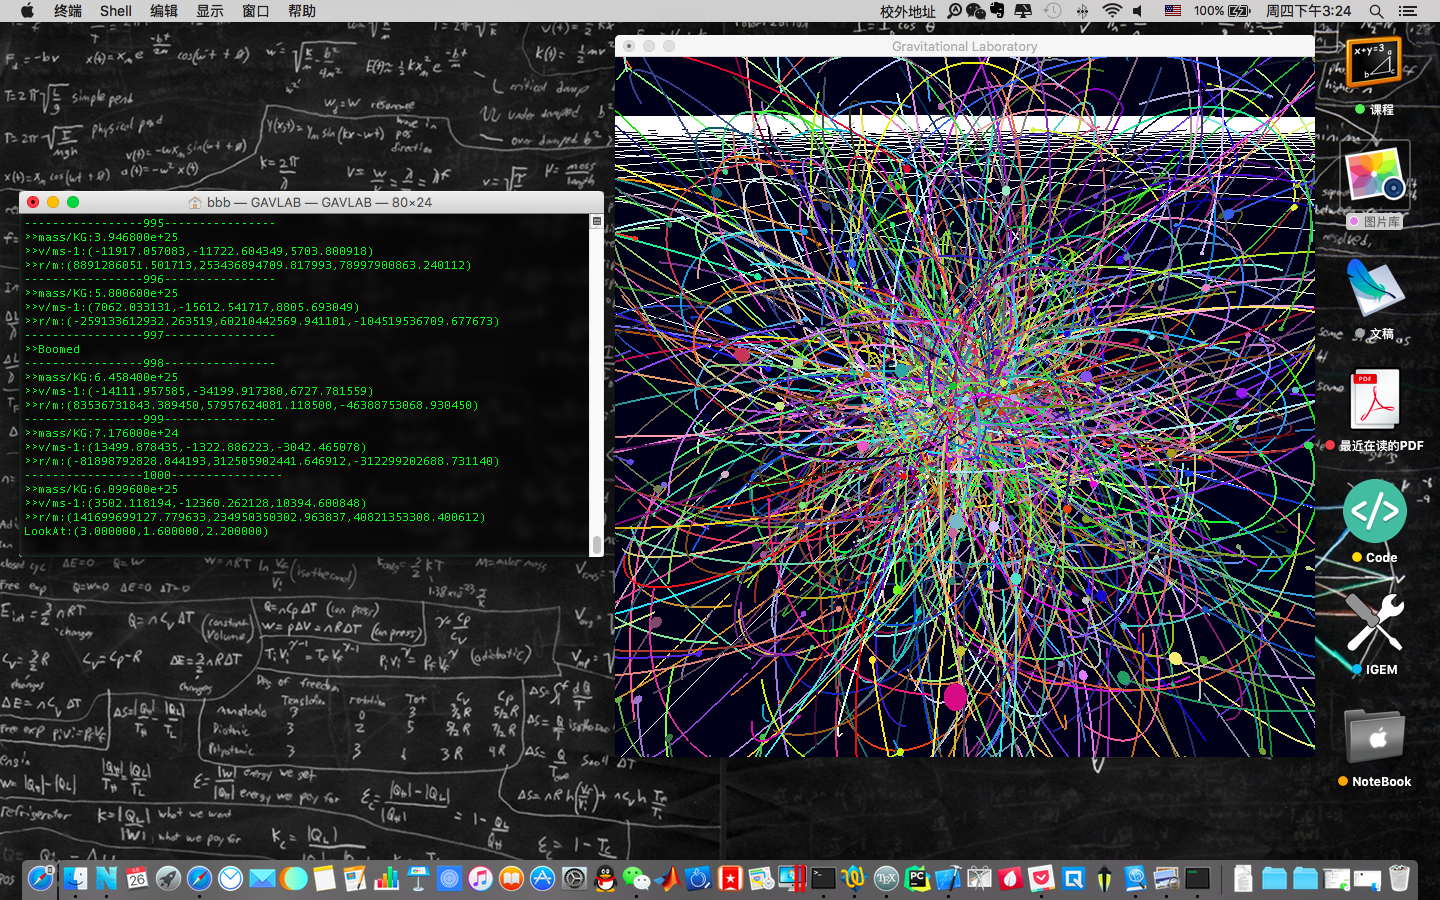
\includegraphics[width=14.4cm,height=9cm]{1000.png}
\end{figure}

\clearpage
\tableofcontents
\clearpage

%%%%%%%%%%%%%%%%%%%%%%%%%%%%%%%%%%%%%%%%%%%%%%%%%%%%%%%%%%%%%%%%%%%%%
\section{Welcome to my Gravitational laboratory}
Hello,welcome to Mr.B's \textbf{G}r\textbf{AV}itational \textbf{LAB}oratory or you can call it \textbf{GAVLAB}.

%>>>>>>>>>>>>>>>>>>>>>>
\subsection{What can you do in GAVLAB} % introduction
Please don't be confused by its name because GAVLAB is not a real laboratory.
Actually it's a virtual laboratory running on computer, a program which can simulate 
the physical process or a system driven by gravitational force.

You can simulate any gravitational process because GAVLAB allows the users to
design their own system in the universe.
In this \textbf{manual mode} users have to set up all information of the system,including the planet's name,mass,radius,position,velocity and RGB color.
It's an exhausting task!

Besides manual mode there are another two automodes for the users who are too busy to set up the system manually.

The first choice is to simulate the \textbf{real solar system} with eight planets in it.
All data was provided by \textbf{Professor Xue} on the website.

The other choice is a little crazy.
It's \textbf{random mode}.
Random mode can generate any number of planets randomly in random position with random velocity and random mass and even random color.
Everything is random!
It means we can simulate hundreds of planets 
by typing several keys on the keyboard and then enjoy the universe and drink a cup of coffee.
It's convenient!
\clearpage

%>>>>>>>>>>>>>>>>>>>>>>

\subsection{How to run GAVLAB}
The first step of running GAVLAB is easy:get a computer.
More specifically, a computer with Linux based system such as MAC with OSX system.

Unfortunately GAVLAB cannot run on Windows system because there are a lot of libraries missing which I will
list out later.

Anyway Mac is the best choice.
On a Mac computer all you have to do is double clicking the executable file named GAVLAB with the sun-shaped logo.

\begin{figure}[H]
\centering

\includegraphics[width=14.4cm,height=9cm]{GAVLAB.png}
\caption{All you have to do to run GAVLAB is double clicking the sun logo}
\end{figure}

%>>>>>>>>>>>>>>>>>>>>>>
\subsection{An illustration of GAVLAB} % figure
It doesn't matter if you don't have a computer with Linux based system because I will demonstrate to you
what GAVLAB looks like when it is running and some results of the experiment in this lab.

\begin{figure}[H]
\centering
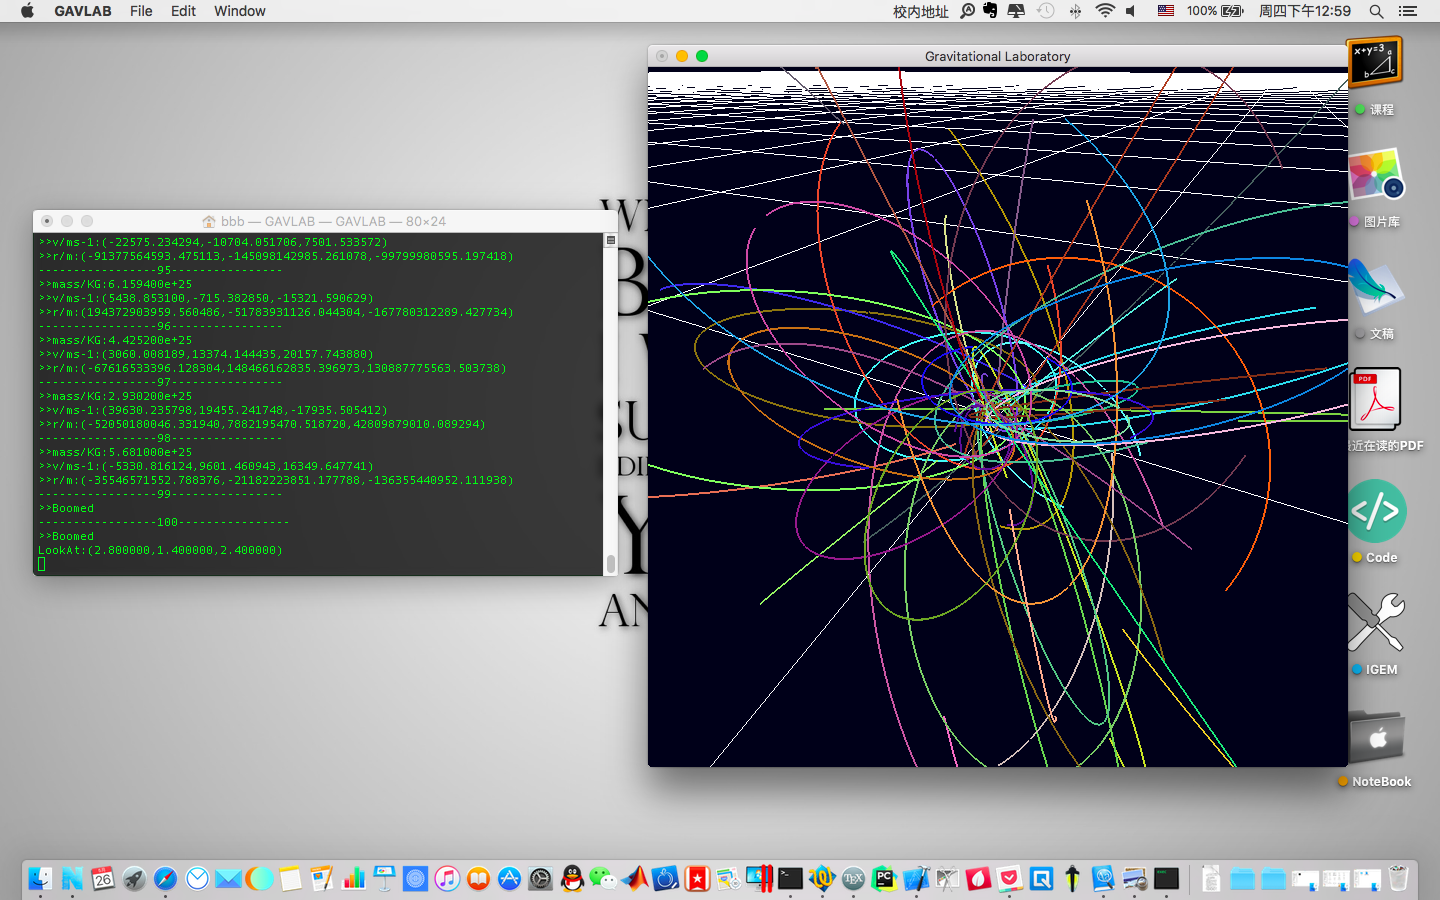
\includegraphics[width=14.4cm,height=9cm]{100.png}
\caption{GAVLAB is simulating a system with 100 planet}
\end{figure}


Figure 1 is the result of simulation of 100 planet.
As you can see those round balls are planets and the colorful lines are their trajectories.

\begin{figure}[H]
\centering
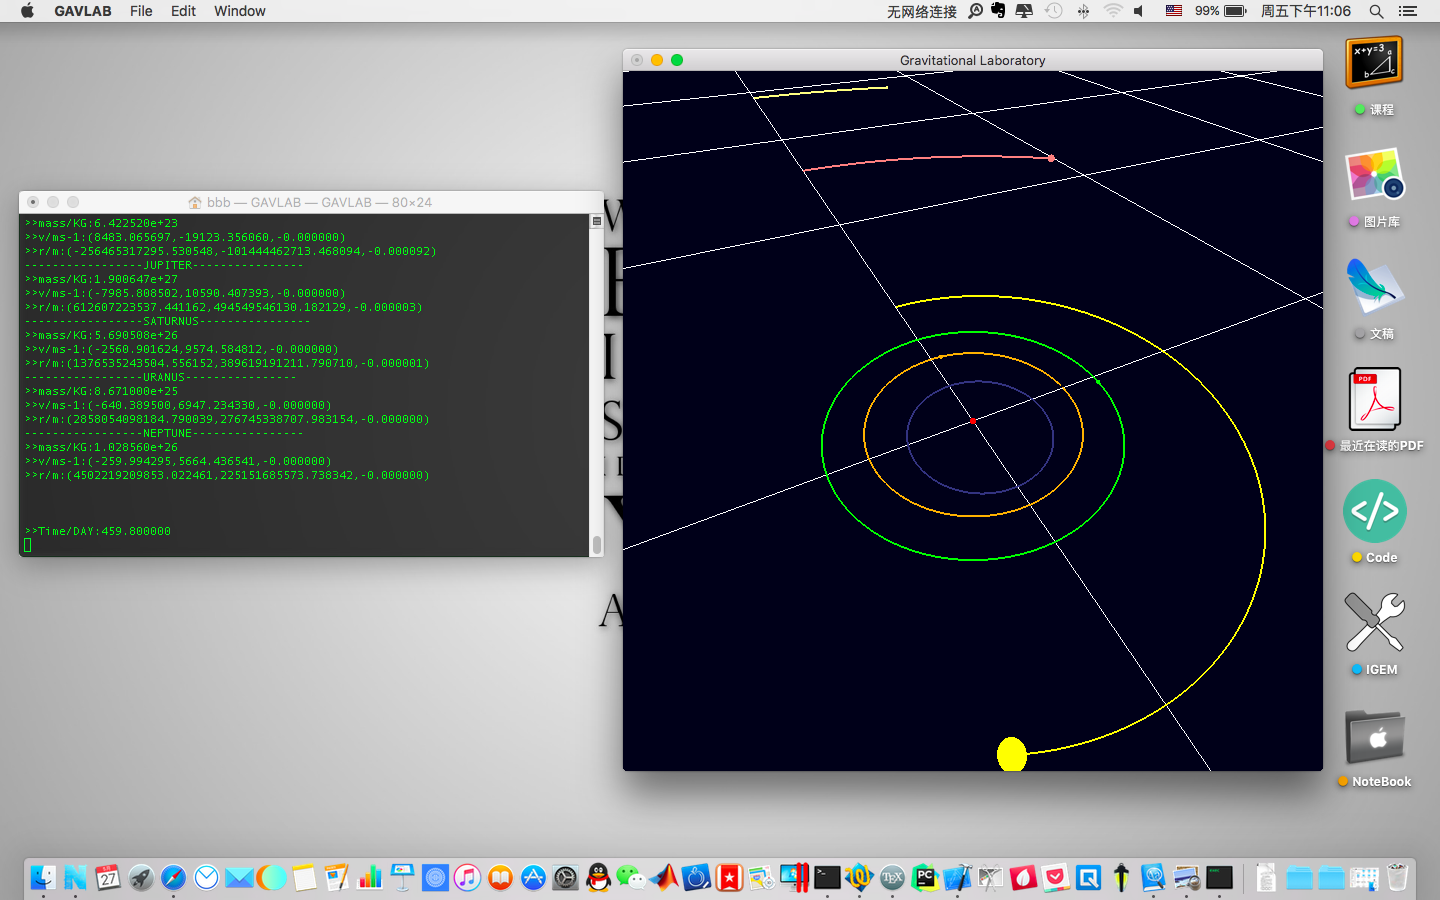
\includegraphics[width=14.4cm,height=9cm]{Solar.png}
\caption{GAVLAB is simulating a real solar system}
\end{figure}

Figure 2 showed the real solar system to you.
It's worth to notice that the trajectory can be really stable as time goes by.
Especially for mercury which it is very close to sun.

\begin{figure}[H]
\centering
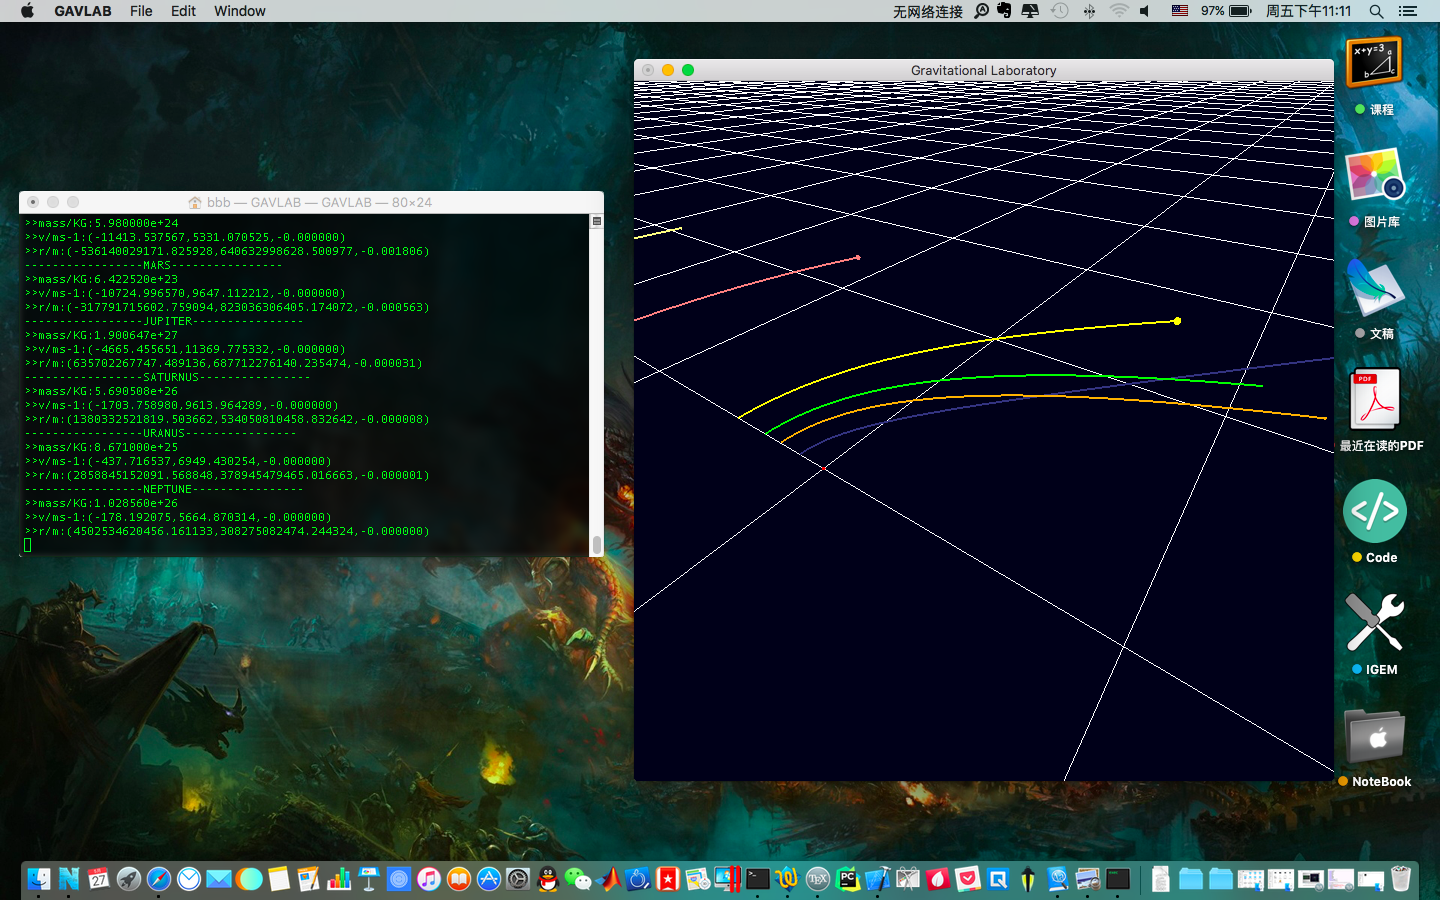
\includegraphics[width=14.4cm,height=9cm]{HalfSolar.png}
\caption{GAVLAB is simulating a half solar system}
\end{figure}

Figure 3 tells you what will happen if half mass of sun dispair.
As you can see some planets will leave the solar system and never come back.
 
\begin{figure}[H]
\centering
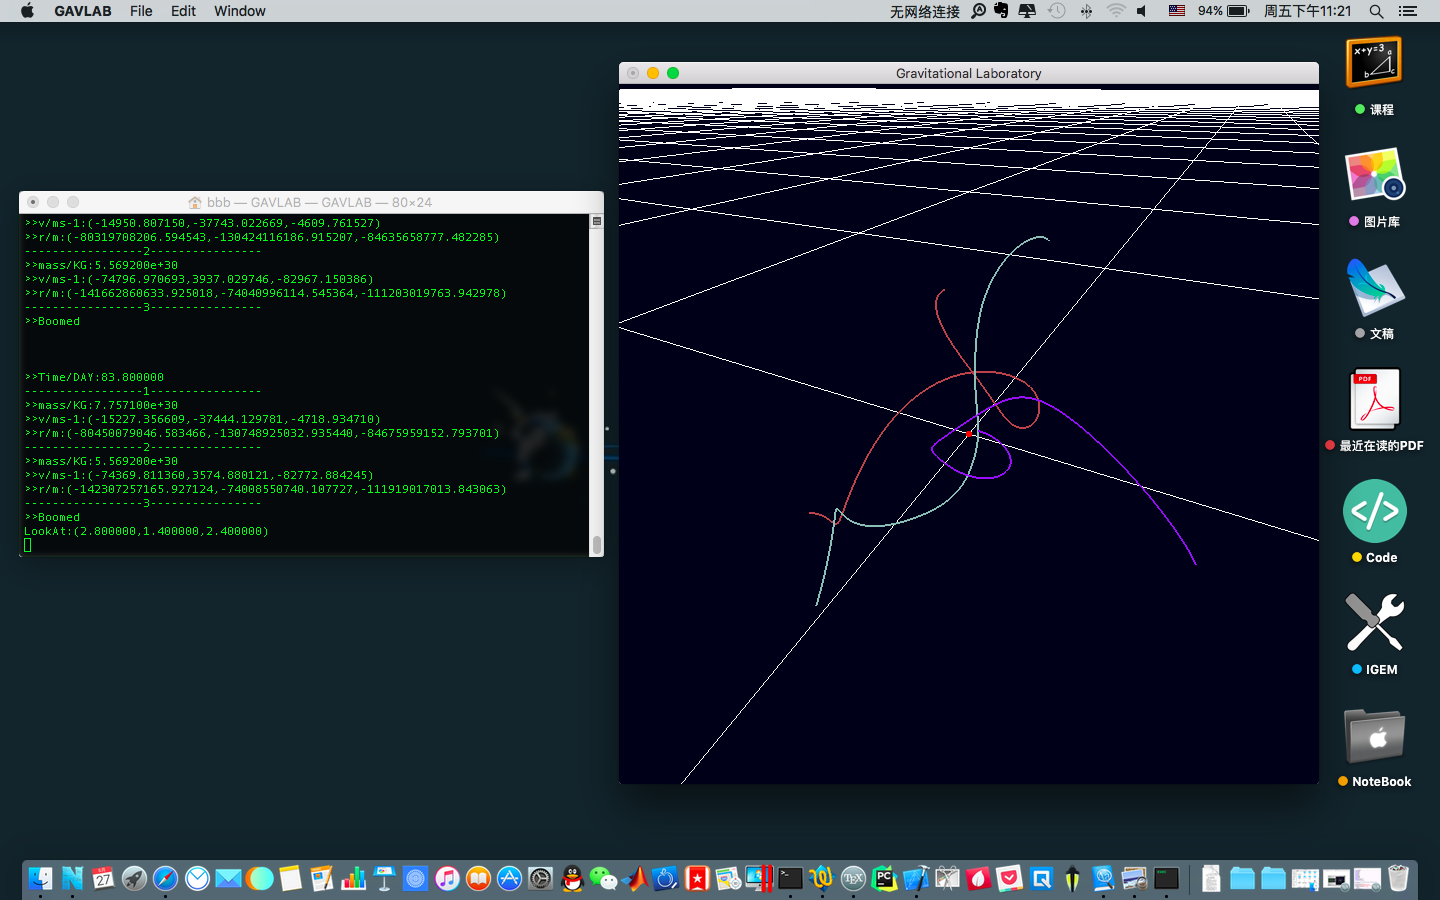
\includegraphics[width=14.4cm,height=9cm]{3Body.png}
\caption{GAVLAB is simulating a 3-body system}
\end{figure}

Figure 4 simulated the 3-body system with equal mass.
What a mess!

\clearpage
%>>>>>>>>>>>>>>>>>>>>>> % summary
\subsection{How was GAVLAB built} 
For geeks and those who love computers and physics I will give you a short summary of how I built GAVLAB.
\subsubsection{Xcode project}
GAVLAB is built on Xcode,an IDE for IOS developers.
On Xcode I can write program in C,C++,objective-C or swift.

The complier of Xcode is Clang developed by Apple Inc.

Xcode is really convenience for programing because it contains lots of functions
such as debugging,breakpoints,code auto complement and beautiful syntax highlight.

Aslo Xcode contains all kinds of libraries such as OpenGL or OpenCL which saved my time setting my developing environment.
\begin{figure}[H]
\centering
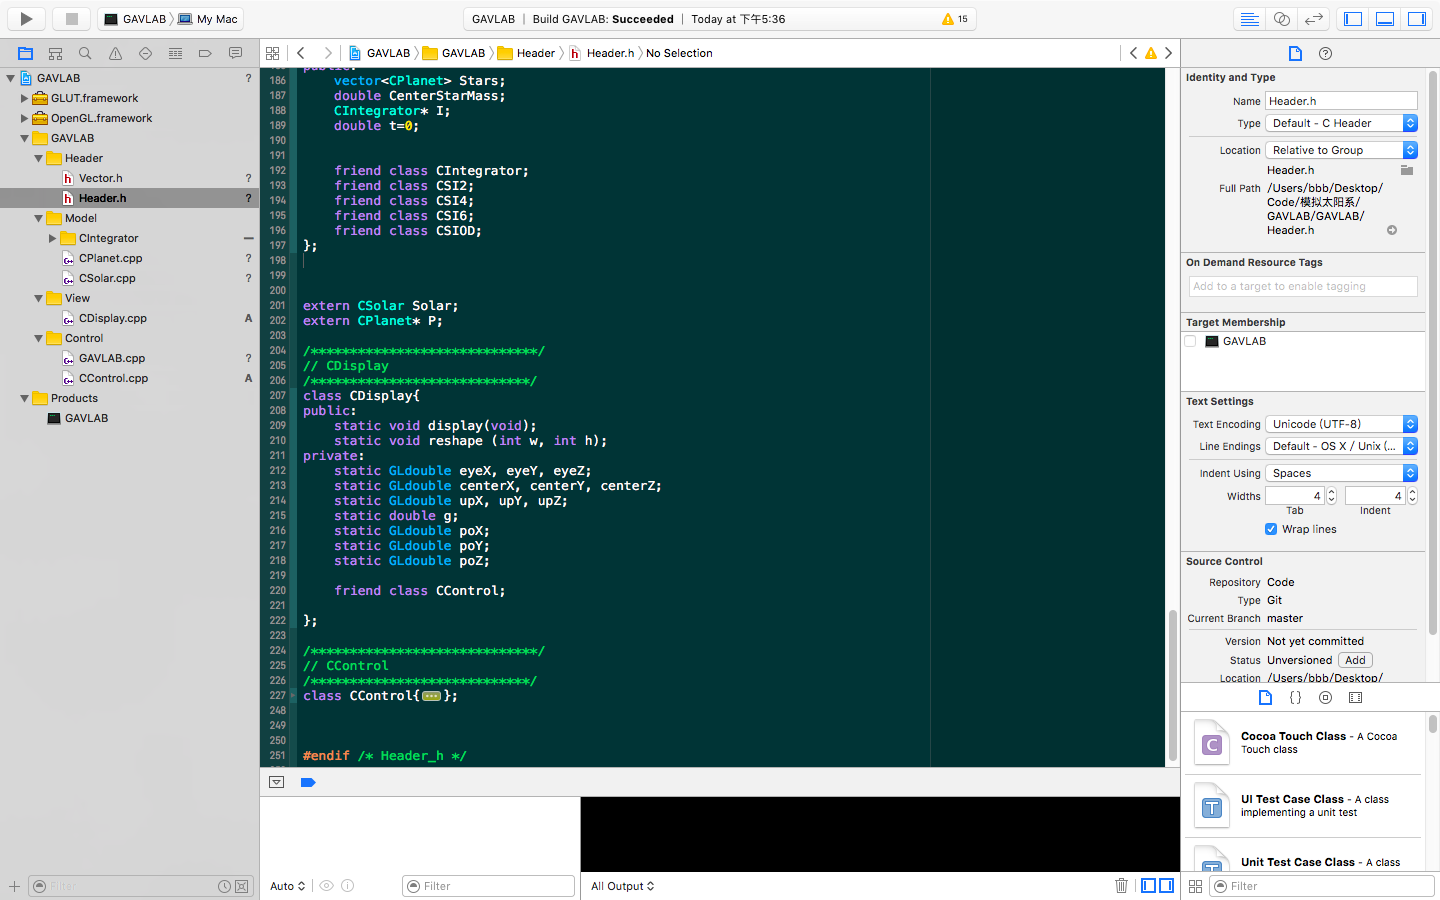
\includegraphics[width=14.4cm,height=9cm]{Xcode.png}
\caption{GAVLAB is an Xcode project}
\end{figure}

\clearpage
\subsubsection{Summary}
GAVLAB was built in C++ language with a little Object-Oriented programing technique.
It contains \textbf{data abstraction},\textbf{inheritance} and \textbf{dynamic binding}.

In GAVLAB each planet is a CPlanet object and the whole solar is a CSolar object which is \textbf{data abstraction}.

There are several kinds of integrators in GAVLAB.
Each of them is an object of class derived from CIntegrator class which is \textbf{inheritance}.

Different integrators share the same method \textbf{Update} with different implementation code which is \textbf{dynamic binding}.

Also I used \textbf{class template} when I was building my math library Vector which is \textbf{generic programing}.

The structure of GAVLAB is \textbf{MVC} where I imitated from the software developing.

Control class takes in charge of the whole program and interact with users in command window.

Model is actually math.
To make our trajectory stable and correct I used \textbf{Symplectic Integrator} with two order,four order and six order.
They can be notated as \textbf{SI2},\textbf{SI4} and \textbf{SI6}.

View method makes GAVLAB visual with OpenGL which is an open graphics API.

\clearpage
% requirement analyses 
%%%%%%%%%%%%%%%%%%%%%%%%%%%%%%%%%%%%%%%%%%%%%%%%%%%%%%%%%%%%%%%%%%%%
\section{What do we need to build GAVLAB}
In this section I will analyze the requirement of building GAVLAB.
\begin{itemize}
\item Data Structure

	\begin{itemize}
		\item We need to store data information of the planet.
		\item We need to divide the space into several grids
	\end{itemize}
\item Model

	\begin{itemize}
		\item We need to make the integrator accurate.
		\item We need to make the energy of the system conserve.
		\item We need to deal with the collision circumstance.
		\item We need to make GAVLAB able to simulate a large amount of planet.
	\end{itemize}
\item Design

	\begin{itemize}
		\item We need to make GAVLAB able to interact with users.
		\item We need to visualize the result of GAVLAB.
		\item We need to make animation while simulating
	\end{itemize}
\end{itemize}




% frame of the program
%%%%%%%%%%%%%%%%%%%%%%%%%%%%%%%%%%%%%%%%%%%%%%%%%%%%%%%%%%%%%%%%%%%%
\section{An overview of GAVLAB's structure }
% MVC
% The figure of the structure
%>>>>>>>>>>>>>>>>
\subsection{MVC}
MVC is Model View and Controller.
Model for GAVLAB here is just simulating the gravitational process.
View is to let the users see the result of the program.
And Controller is the commander which takes the command of users and tells the program what to do.

In GAVLAB there will be a loop.
At the beginning of each loop the Controller will get the command of the users such as starting simulation or pause.
Then it parses the command and execute the command.

After that the model will simulate the physics process according the integrator and update the state.

Finally View is responsible for making the animation according the data generated by model.
%>>>>>>>>>>>>>>>>
\clearpage
\subsection{Illustration}
This is the illustration figure of the structure.
\begin{figure}[H]
\centering
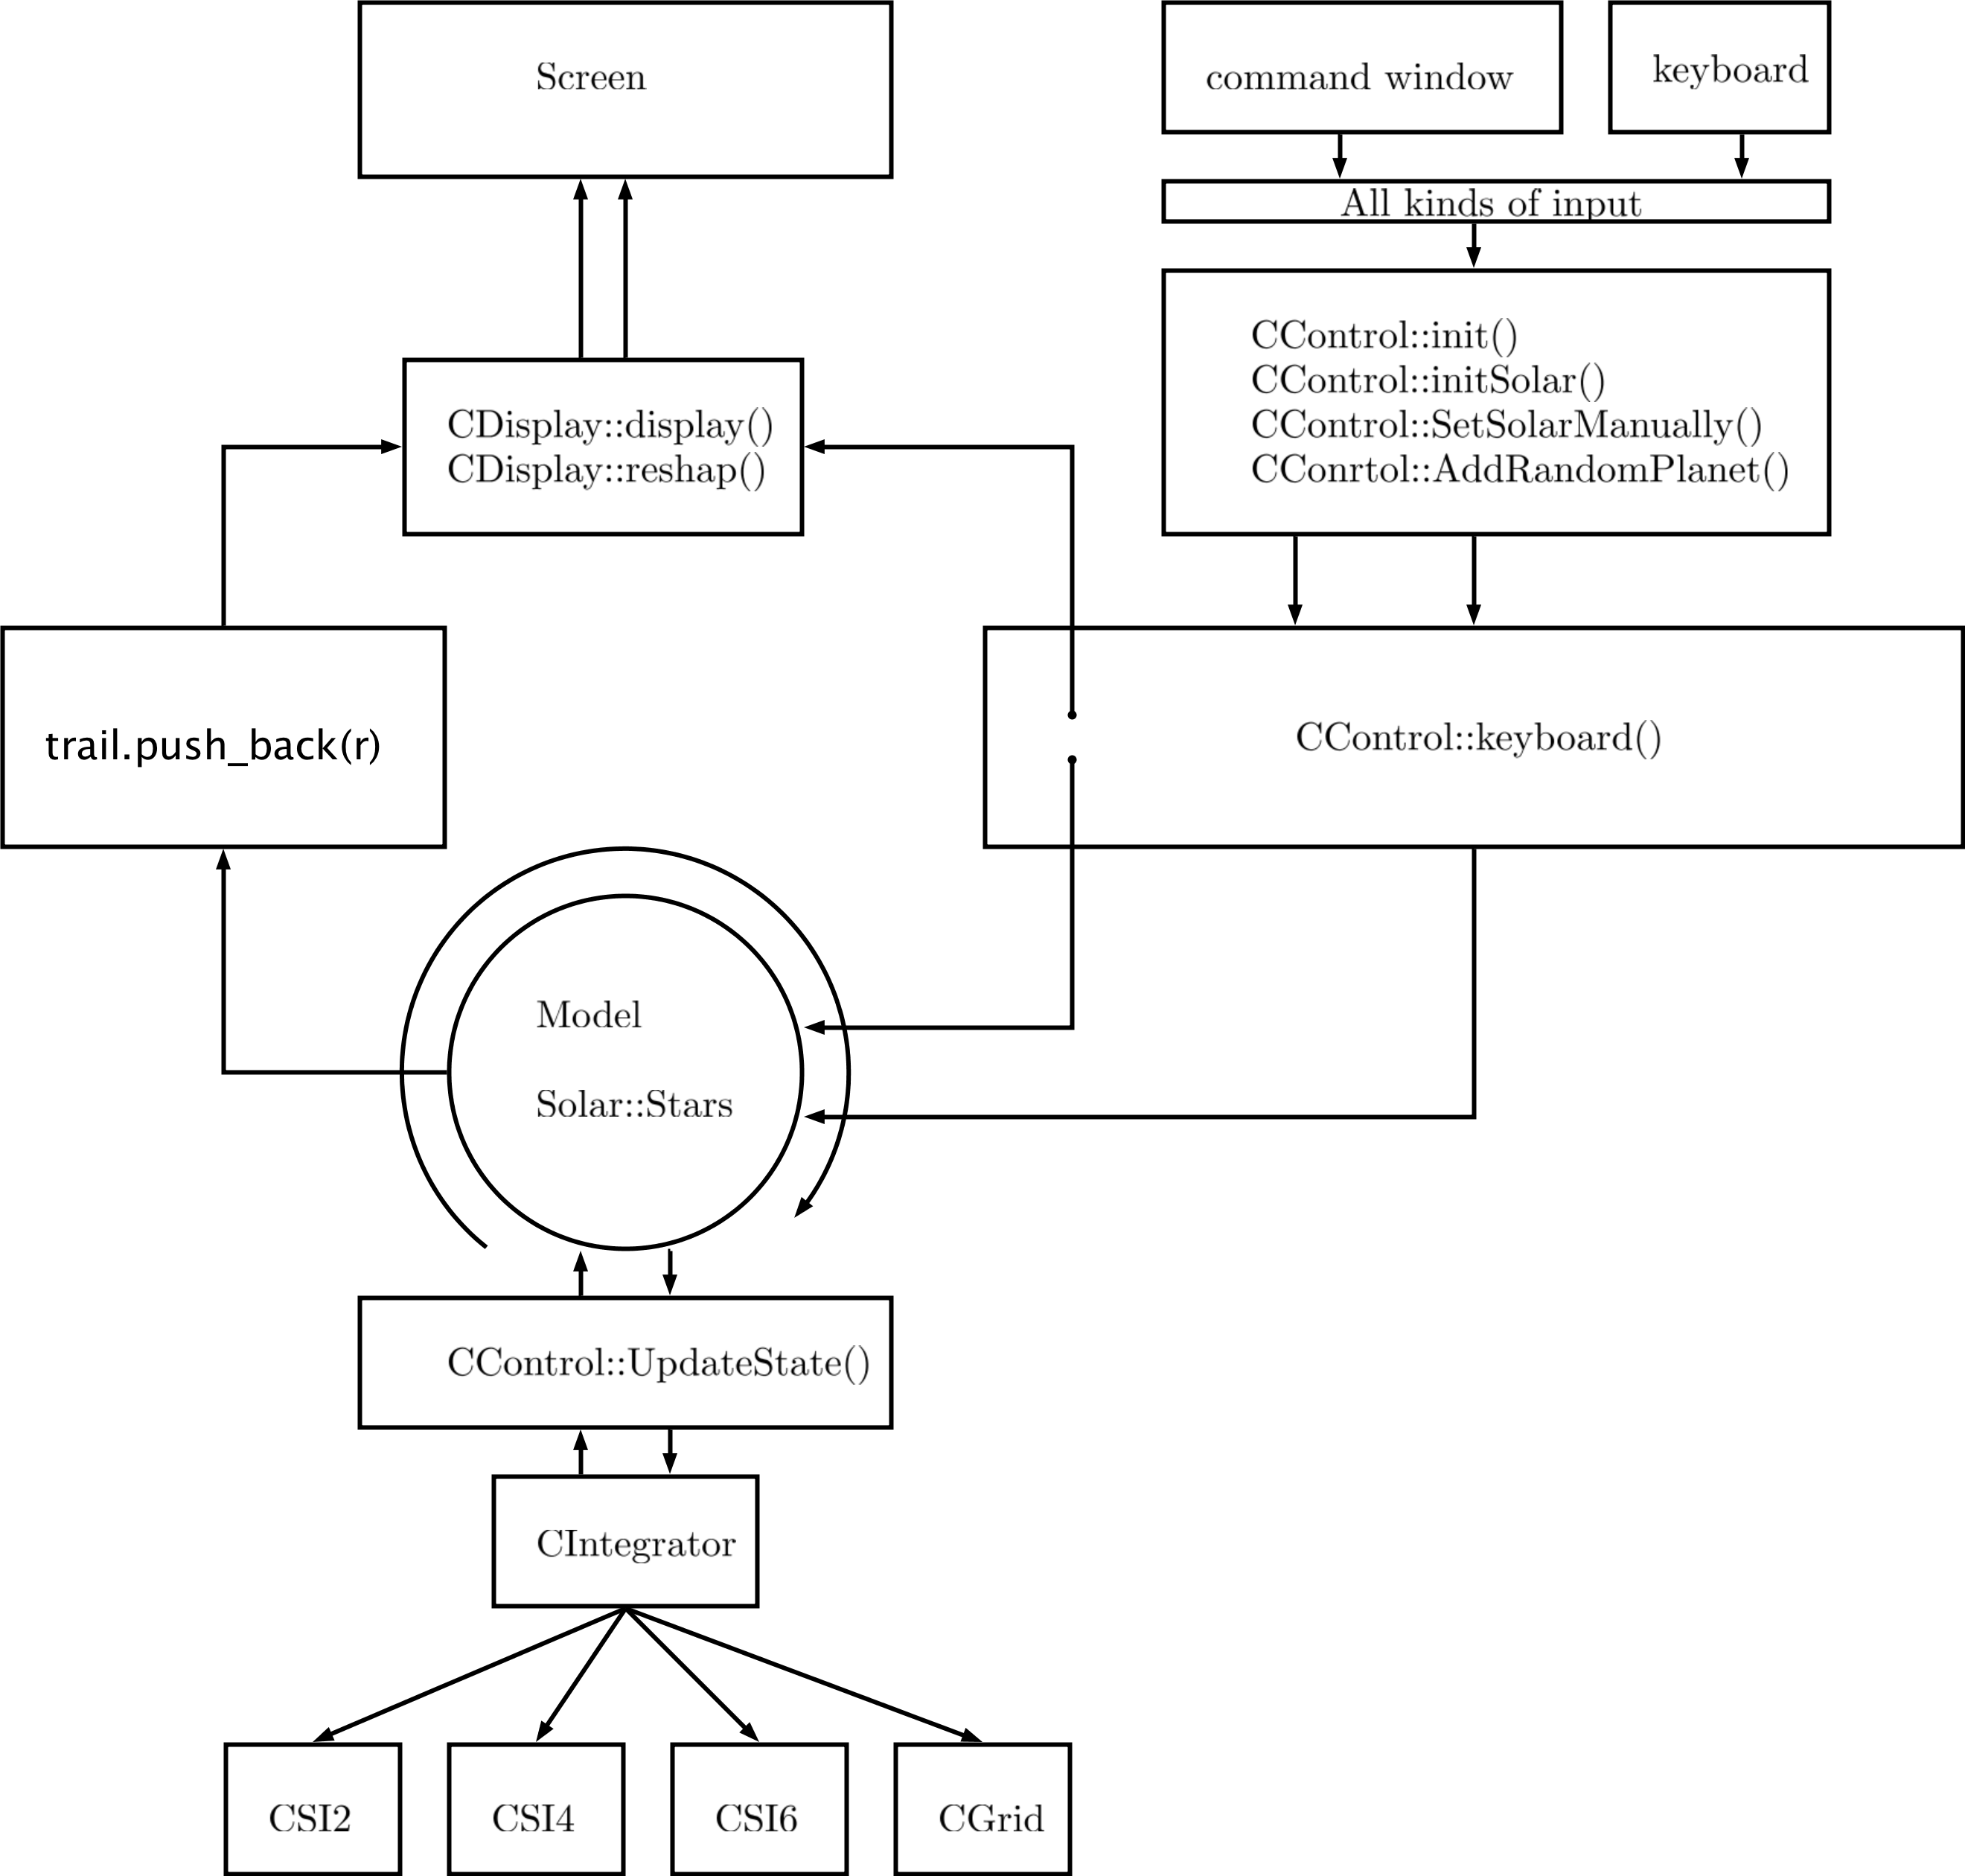
\includegraphics[width=13.2cm,height=12.6cm]{frame.png}
\caption{GAVLAB has a frame similar to MVC}
\end{figure}

%>>>>>>>>>>>>>>>>>>
\clearpage
\subsection{Structure of program}
\begin{description}[align=left]
\item [$\complement$ Header] Folder contains two header files
	\begin{description}[align=left]
	\item [$\boxplus$ Header.hpp] Header file contains declarations of all the classes
		\begin{description}[align=left]
		\item [$\blacktriangleright$ class CIntegrator] Base class of all integrators
		\end{description}
	\item [$\boxplus$ Vector.hpp] Math Library contains all kinds of vector operation
		\begin{description}[align=left]
		\item [$\blacktriangleright$ class Vector$<class T>$] Vector template
		\end{description}
	\end{description}
\item [$\complement$ Model] Folder contains model related files
	\begin{description}[align=left]
	\item [$\complement$ CIntegrator] Folder contains all the integrators
		\begin{description}[align=left]
		\item [$\boxplus$ CSI2.cpp] 2-order Symplectic Integrator 
			\begin{description}[align=left]
			\item [$\blacktriangleright$ class CSI2] 
			\end{description}
		\item [$\boxplus$ CSI4.cpp] 4-order Symplectic Integrator
			\begin{description}[align=left]
			\item [$\blacktriangleright$ class CSI4] 
			\end{description}
		\item [$\boxplus$ CSI6.cpp] 6-order Symplectic Integrator
			\begin{description}[align=left]
			\item [$\blacktriangleright$ class CSI6] 
			\end{description}
		\item [$\boxplus$ CGrid.cpp] Grid method
			\begin{description}[align=left]
			\item [$\blacktriangleright$ class CGrid] 
			\end{description}
		\end{description}
	\item [$\boxplus$ CPlanet.cpp] File contains definition of CPlanet class
		\begin{description}[align=left]
		\item [$\blacktriangleright$ class CPlanet] class to store Planet's information
		\end{description}
	\item [$\boxplus$ CSolar.cpp] Folder contains definition of CSolar class
		\begin{description}[align=left]
		\item [$\blacktriangleright$ class CSolar] class to represent the whole solar system
		\end{description}
	\end{description}
\item [$\complement$ View] Folder contains View related files
	\begin{description}[align=left]
	\item [$\boxplus$ CDisplay.cpp] File contains definition of CDisplay class
		\begin{description}[align=left]
		\item [$\blacktriangleright$ class CDisplay] Contains OpenGL code to make animation
		\end{description}
	\end{description}
\item [$\complement$ Control] Folder contains Controller related files
	\begin{description}[align=left]
	\item [$\boxplus$ CControl.cpp] File contains definition of CControl class
		\begin{description}[align=left]
		\item [$\blacktriangleright$ class CControl] class control the input and parse command
		\end{description}
	\item [$\boxplus$ GAVLAB.cpp] File contains main function
		\begin{description}[align=left]
		\item [$\blacktriangleright$ int main()] main function runs the Loop
		\end{description}
	\end{description}
\end{description}
% CODE HERE
%>>>>>>>>>>>>>
\section{MODEL is actually math}
%>>>>>>>>>>>>>
\subsection{Math Library Vector}
We are physicists and we prefer writing our equation in concise form.
So there will be a lot of vector and matrix operation in our equations and formulas.
Especially in Newton's Law and the formula of gravity force there are vectors.

For that reason it will save us a lot of time if we define our own \textbf{Vector} operation
library\cite{mathlibrary}.Here's my code of class template Vector
\begin{lstlisting}[caption=Vector Library I]
template<class T>
class Vector{
public:
    explicit Vector(T a=0,T b=0,T c=0):x{a},y{b},z{c}{};
    Vector(const Vector<T>& u)=default;
    Vector(Vector<T> && u)=default;
    Vector<T>& operator=(const Vector<T>&u)=default;
    Vector<T>& operator=(Vector<T>&&u)=default;
    T Magnitude(void);
    Vector<T>  Normalize(void);
    Vector<T>  Reverse(void);
    // vector operation
    Vector<T>& operator+=(const Vector<T> &u);
    Vector<T>& operator-=(const Vector<T> &u);
    // scaler operation
    Vector<T>& operator*=(T s);	
    Vector<T>& operator/=(T s);	
    bool operator ==(const Vector<T> &u);
    bool operator !=(const Vector<T> &u);
    inline T X()const{return x;}
    inline T Y()const{return y;}
    inline T Z()const{return z;}
\end{lstlisting}
\clearpage
\begin{lstlisting}[caption=Vector Library II]
friend Vector<T> operator+<>(const Vector<T>& u,const Vector<T> &v);
friend Vector<T> operator-<>(const Vector<T>& u,const Vector<T> &v);
friend Vector<T> operator^<>(const Vector<T>& u,const Vector<T> &v);
friend T operator*<>(const Vector<T>& u,const Vector<T> &v);
friend Vector<T> operator*<>(T s, const Vector<T>& u);
friend Vector<T> operator*<>(const Vector<T>& u, T s);
friend Vector<T> operator/<>(const Vector<T>& u, T s);
friend ostream& operator<< <>(ostream &out,const Vector<T>& u);
private:
    T x,y,z;
};
\end{lstlisting}

Those methods are just ordinary math formula for basic vector operation which is very trivial.
So I will not show the implementations of those methods.
Instead I will show my type definition of template class Vector

\begin{lstlisting}[caption=typedef]
// Vector with three float type variables
typedef Vector<float> vector3f;
// Vector with three double type variables
typedef Vector<double> vector3d;
\end{lstlisting}
\clearpage
\subsection{CPlanet class}
To store and manage the data of each planet we can abstract the planet to be an object.
So I defined CPlanet class.

\begin{lstlisting}[caption=CPlanet class I]
class CPlanet{
public:// Constructor
    CPlanet(string name, 
            double mass,
            double radius,
            double x,double y,double z,
            double vx,double vy,double vz,
            double Red,double Green,double Blue):
Name(name), Mass(mass),Radius(radius),r(vector3d(x,y,z)),v(vector3d(vx,vy,vz))
,Color(vector3d(Red,Green,Blue)){exist=true;}
    // Get the attribute
    inline const vector3d& GetR()const{return r;}
    inline const vector3d& GetV()const{return v;}
    inline const double X()const{return r.X();}
    inline const double Y()const{return r.Y();}
    inline const double Z()const{return r.Z();}
    double GetMass()const{return Mass;}
    inline string GetName()const{return Name;}
    inline const double Red()const{return Color.X();}
    inline const double Green()const{return Color.Y();}
    inline const double Blue()const{return Color.Z();}
    inline const bool Exist()const{return exist;}
    inline const double GetRadius()const{return Radius;}
\end{lstlisting}
\clearpage
\begin{lstlisting}[caption=CPlanet class II]
    // Set the attribute
    void SetR(double a,double b,double c){r=vector3d(a,b,c);}
    void SetV(double a,double b,double c){v=vector3d(a,b,c);}
    // update the state
    void Updatetr(double DT){trail.push_back(r);}
    // list storing trajectory
    list<vector3d> trail;
private:
    double Mass;
    string Name;
    double Radius;
    vector3d r;
    vector3d v;
    vector3d Color;
    bool exist; // false if it explode
    
    friend class CSolar;
    friend class CIntegrator;
    friend class CSI2;
    friend class CSI4;
    friend class CSI6;
    friend class CGrid;
};
\end{lstlisting}

Not too much complicated method for CPlanet because it's just a data structure
to store the data.
It contains the name,mass,radius,position,velocity,color and a bool type variable representing if it exists.

In GAVLAB we don't really delete the CPlanet object if it has exploded 
because we want to plot the trajectory of every planet and research how it exploded
or which planet it collided with.
So we just use a bool type flag called exist to mark that information.
\clearpage
\subsection{CSolar class}
We have a lot of operation aimed at the whole solar system so it's good to abstract that system
as an object too.
We defined CSolar system to store all CPlanet and the complicated method or algorithm interface.

\begin{lstlisting}[caption=CSolar class]
class CSolar{
public:// Constructor
    CSolar(double mass):CenterStarMass(mass){ }
    CSolar(){}
    // Set the attribute
    void SetMass(double mass){CenterStarMass=mass;}
    void SetI(int command);
    void SetStep(double DT_){I->SetDT(DT_);}
    // Get the attribute
    double GetMass()const {return CenterStarMass;}
    double GetT()const{return t;}
    bool AddPlanet(CPlanet &P);// Method
    void GenerateRandomPlanet();// Method
    void UpdateSolar();// Method
public:
    vector<CPlanet> Stars;
    double CenterStarMass;
    CIntegrator* I;
    double t=0; 
    friend class CIntegrator;
    friend class CSI2;
    friend class CSI4;
    friend class CSI6;
    friend class CGrid;
};
\end{lstlisting}

The CSolar class has a vector member containing all the planet object in it.
Besides that we need to store the center mass of the solar for our convenience of adjusting that.


\clearpage
The most important member I is the integrator which I'll explain later.
For now we just know each solar can have one integrator to update the state 
and they are all inherited from the base class CIntegrator.

\begin{lstlisting}[caption=SetI() ]
void CSolar::SetI(int command){
    switch (command) {
        case SI2:
            I = new CSI2;
            break;
        case SI4:
            I = new CSI4;
            break;
        case SI6:
            I = new CSI6;
            break;
        case Grid:
            I = new CGrid;
            break;
        default:
            break;
    }   
}
\end{lstlisting}
here SI2 SI4 ... are macro defined int type variables in Header.h

Also adding a planet into the solar is an important method.
\begin{lstlisting}[caption=AddPlanet()]
bool CSolar::AddPlanet(CPlanet &P){
    Stars.push_back(P);
    return true;
}
\end{lstlisting}
\clearpage
To generate random solar system we need to generate random planet to the solar.
\begin{lstlisting}[caption=GenerateRandomPlanet()]
int Number=1;
void CSolar::GenerateRandomPlanet(){
    srand((unsigned)time(0));
    char S[10];
    sprintf(S, "%d",Number++);
    string name=S;
    double mass=double(arc4random()%100+10);
    mass*=(ME/10); 
    double radius=double(arc4random()%10+1);
    radius/=10.0;
    double x=double(arc4random()%20+1)*flag();
    double y=double(arc4random()%20+1)*flag();
    double z=double(arc4random()%20+1)*flag();
    x*=(0.1*RA);y*=(0.1*RA);z*=(0.1*RA);
    double vx=double(arc4random()%100+10)*flag();
    vx*=100;
    double vy=double(arc4random()%100+10)*flag();
    vy*=100;
    double vz=double(arc4random()%100+10)*flag();
    vz*=100;
    double r=double(arc4random()%100+1);
    r/=100.0;
    double b=double(arc4random()%100+1);
    b/=100.0;
    double g=double(arc4random()%100+1);
    g/=100.0;
    P = new CPlanet(name,mass,radius,x,y,z,vx,vy,vz,r,g,b);
    AddPlanet(*P);
}
\end{lstlisting}

\clearpage
Further more we have to Update the solar system.
\begin{lstlisting}[caption=UpdateSolar()]
void CSolar::UpdateSolar(){
    I->Update(*this);// call method of integrator
    // check for collision
    vector<CPlanet>::iterator itri,itrj;
    for (itri=Stars.begin(); itri != Stars.end(); itri++) {
        if (itri->exist == false) {continue;}
        double R0=(itri->r^(itri->v/(itri->v.Magnitude()))).Magnitude();
        if (R0<E) {// if it passed the sun
            cout<<itri->Name<<" BOOM"<<endl;
            itri->exist=false;
        }
        for (itrj=Stars.begin(); itrj!=Stars.end(); itrj++) {
            if (itrj == itri || itrj->exist==false) {
                continue;
            }
            vector3d rij=itri->r-itrj->r;
            double R=rij.Magnitude();
            if(R < E){// if the planets are close
                cout<<itri->Name<<" and "<<itrj->Name<<" BOOM!"<<endl;
                itri->v=(itri->Mass*itri->v+itrj->Mass*itrj->v)/(itri->Mass+itrj->Mass);
                itri->Mass+=itrj->Mass;
                itrj->exist=false;       
            }
        }
    }
}
\end{lstlisting}

%>>>>>>>>>>>>>
\subsection{Integrator is important}
As we know almost all GAVLAB has to do is simulating.
Because the real physics world is driven by differential equation such as Newton's Law
or Hamiltonian equation, GAVLAB has to integrate those equations to get the solution.
So we need a good integrator.

There's something different between computer simulation and real world's physical process.
In computer we can only solve \textbf{difference equations} rather than \textbf{differential equations}
because computers can only deal with decrete math.
So instead of calculating infinitesimal step time we have to calculate the new state of the system after 
some pretty small but finite time step $\tau$.Then if $\tau$ is too large it will lose accuracy.

There're some good integrators such as Euler method or Runge-Kutta method.
However those methods are not suitable in GAVLAB cause we want our trajectory stable.
It's easy to know that the deviation of energy will increase as time goes through using Euler or Runge-Kutta method
which means the radius of planet's trajectory will decrease slowly and finally move to sun.

So in GAVLAB I used \textbf{Symplectic Integrating}\cite{SI} method which is able to maintain the \textbf{symplectic proporty} of 
the planet's canonical coordinate and canonical momentum $(q,p)$.

%>>>>>>>>>>>>>
\subsection{CIntegrator}
Here is the code of CIntegrator,base class of all the integrators.

\begin{lstlisting}[caption=CIntegrator]
class CIntegrator{
protected:
    double DT;//time step
public:
    virtual void Update(CSolar &S)=0;
    void SetDT(double dt){DT = dt;}
    double GetDT()const{return DT;}
};
\end{lstlisting}

In CIntegrator class we have pure virtual function Update which means
CIntegrator is abstract class.

\subsection{Quick description of Symplectic Integrator}
It is easy to know that the gravitational system is separable Hamilton system which means
Hamiltonian $H(p,q)$ can be written as
\begin{equation}
H(p,q)=T(p)+V(q)
\end{equation}

And we have Hamilton equation of motion:
\begin{equation}
\begin{aligned}
\dot{p}&=-\frac{\partial V}{\partial q} =\varphi (q)\\
\dot{q}&=\frac{\partial T}{\partial p} =\phi (p)
\end{aligned}
\end{equation}


So according to Hamilton equation's difference form we give the difference equation of 
Symplectic Integrator here:
\begin{equation}
\begin{aligned}
q(t_{k}) &= q(t_{k-1}) +\tau\sum_{i=1}^{m}c_{i}\phi_{i-1} \\
p(t_{k}) &= p(t_{k-1}) +\tau\sum_{i=1}^{m}d_{i}\varphi_{i}
\end{aligned}
\end{equation}
Where $m$ is the order of integration and $c_{i}$ $d_{i}$ are some specific coefficients.

The form of $\phi_{i-1}$ and $\varphi_{i}$ is
\begin{equation}
\begin{aligned}
\phi_{i-1}&=\phi (p^{i-1}) \\
\varphi_{i}&=\varphi (q^{i})
\end{aligned}
\end{equation}

And we used $m$ assist points $(p^i,q^i)$ in the difference form equation.
Here is how they are represent
\begin{equation}
\begin{aligned}
q^i &= q^{i-1} + \tau c_{i} \phi (p^{i-1}) \\ 
p^i &= p^{i-1} + \tau d_{i} \varphi (q^{i}) \quad (i=1,2\dots m)
\end{aligned}
\end{equation}
%>>>>>>>>>>>>>
particularly here we have
\begin{equation}
\begin{aligned}
p^0 &= p(t_{k-1}) \quad p^m=p(t_{k}) \\ 
q^0 &= q(t_{k-1}) \quad q^m=q(t_{k}) 
\end{aligned}
\end{equation}

Now I'll show you the equations and code of CSI2,CSI4 and CSI6.

\clearpage
\subsubsection{CSI2}
This is the definition of class CSI2 
\begin{lstlisting}[caption=CSI2 class]
class CSI2:public CIntegrator{
public:
    void Update(CSolar &S);
};
\end{lstlisting}

Actually SI2 is just Leap Frog algorithm.
\begin{equation}
\begin{aligned}
q^{*} &= q(t_{k-1}) + \frac{\tau}{2}\left( \frac{\partial T}{\partial p}\right)_{p=p(t_{k-1})} \\ 
p(t_{k}) &= p(t_{k-1}) - \frac{\tau}{2}\left( \frac{\partial V}{\partial q}\right)_{q=q^{*}} \\
q(t_{k}) &= q(t_{k-1}) + \frac{\tau}{2}\left( \frac{\partial T}{\partial p}\right)_{p=p(t_{k})}
\end{aligned}
\end{equation}
here $c_{1}=c_{2}=\frac{1}{2}\quad d_{1}=1\quad d_{2}=0$

\begin{lstlisting}[caption=CSI2 Part I]
void CSI2::Update(CSolar &S){
    vector<CPlanet>::iterator itri,itrj;
    for (itri = S.Stars.begin(); itri != S.Stars.end(); itri++) {
        if (itri->Exist() == false) {continue;}
        vector3d r_;
        r_ = itri->r+0.5*DT*(itri->v);
        vector3d v_=itri->v;
        double R_ = r_.Magnitude();
        v_ -=DT*G*S.GetMass()*r_/(R_*R_*R_);
        for (itrj = S.Stars.begin(); itrj != S.Stars.end(); itrj++) {
            if(itri == itrj || itrj->Exist() == false) continue;
\end{lstlisting}
\begin{lstlisting}[caption=CSI2 Part II]
            vector3d rij = r_ - itrj->r;
            double R = rij.Magnitude();
            v_ -= DT*G*itrj->GetMass()*rij/(R*R*R);
        }
        itri->v = v_;
        itri->r +=0.5*DT*v_;
        itri->Updatetr(DT);
    }
    S.t+=DT;
}
\end{lstlisting}

And here's the how SI2 works

\begin{figure}[H]
\centering
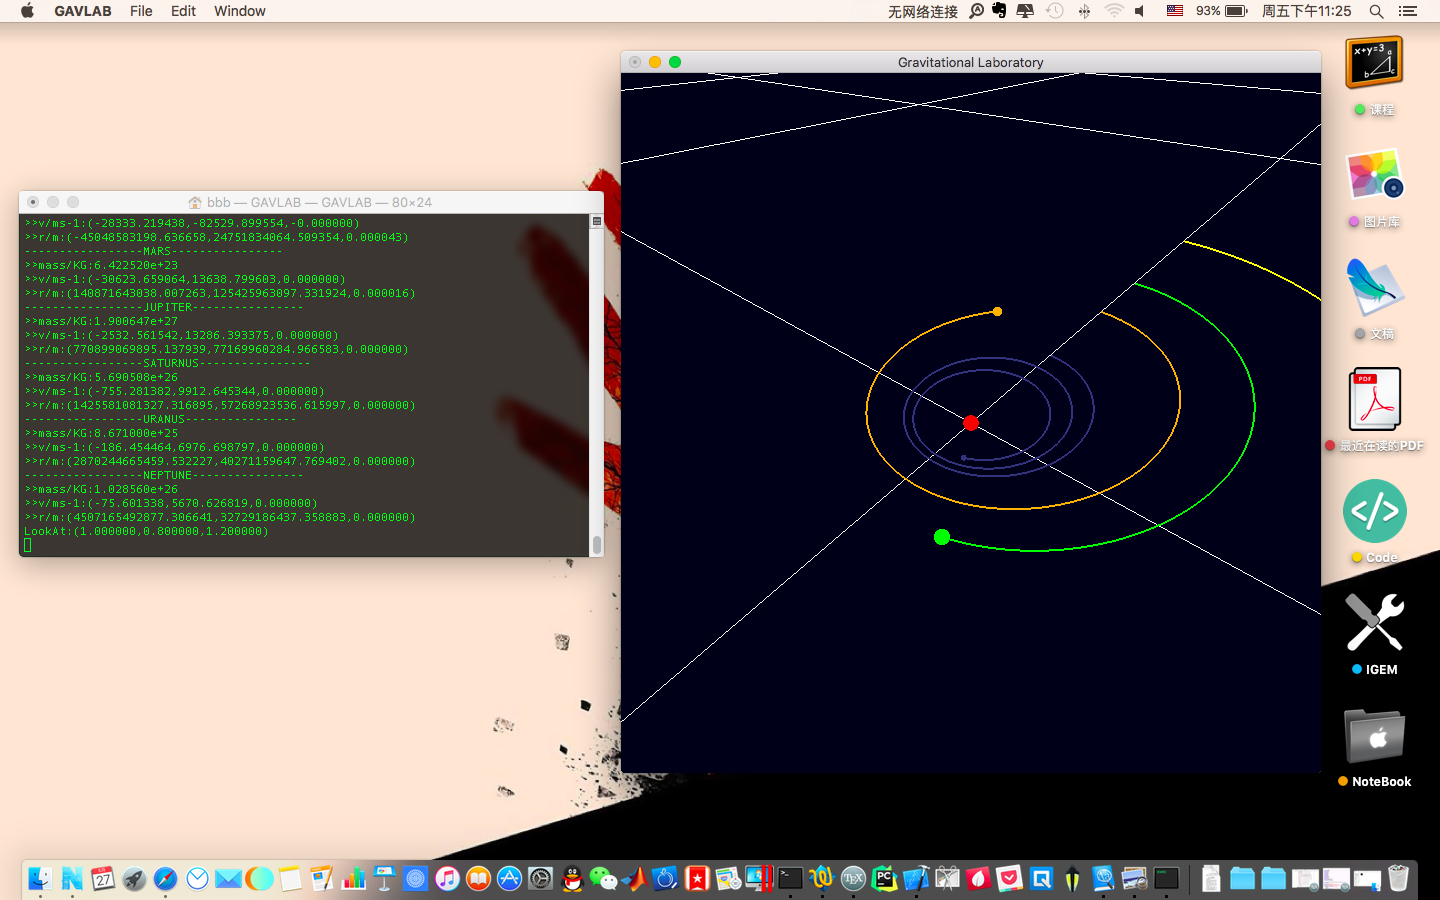
\includegraphics[width=14.4cm,height=9cm]{SI2.png}
\caption{GAVLAB is simulating solar system with SI2}
\end{figure}

As you can see SI2(LeapFrog method) is not pretty stable for trajectory.
The energy of planet will decrease as time goes by and finally fall into sun.
So we have to increase the order of integration to get more precise solution.


\clearpage
\subsubsection{CSI4}
This is the definition of class CSI4
\begin{lstlisting}[caption=CSI4 class]
class CSI4:public CIntegrator{
public:
    void Update(CSolar &S);
};
\end{lstlisting}

The formula of SI4 was derived by Neri\cite{SI4} in 1987 and the difference equation is
\begin{equation}
\begin{aligned}
q^i &= q^{i-1} + \tau c_{i} \frac{\partial T}{\partial p}\left(p^{i-1} \right) \\
p^i &= p^{i-1} - \tau d_{i} \frac{\partial V}{\partial q}\left(q^{i} \right) \quad i=1,2\dots 4
\end{aligned}
\end{equation}
here the coefficient is
\[
\begin{aligned}
c_{1} &= c_{4}=\frac{1}{2(2-\sqrt[3]{2})},\quad c_{2}=c_{3}=\frac{1-\sqrt[3]{2}}{2(2-\sqrt[3]{2})}\\
d_{1} &= d_{3}=\frac{1}{2-\sqrt[3]{2}},\quad d_{2}=c_{3}=-\frac{\sqrt[3]{2}}{2-\sqrt[3]{2}},\quad d_{4}=0
\end{aligned}
\]

Here's code
\begin{lstlisting}[caption=CSI4 Part I]
void CSI4::Update(CSolar &S){
    
    double c[5]={0,0.67560359597,-0.1756035979,
    -0.1756035979,0.67560359597};
    double d[5]={0,1.3512071919596577,
    -1.70241438391932,1.3512071919596577,0};
    vector<CPlanet>::iterator itri,itrj;
    for (itri = S.Stars.begin(); itri != S.Stars.end(); itri++) {
        if (itri->exist==false) {continue;}
\end{lstlisting}
\begin{lstlisting}[caption=CSI4 Part II]
        vector3d r_[5],v_[5];
        r_[0]=itri->r;
        v_[0]=itri->v;
        for (int i=1; i<=4; i++) {
            r_[i]=r_[i-1] + DT*c[i]*v_[i-1];
            // Center gravity
            double r=r_[i].Magnitude();
            v_[i] = v_[i-1]-G*DT*d[i]*S.GetMass()*r_[i]/(r*r*r);
            if(i == 4) continue;
            // gravity between stars
            for (itrj = S.Stars.begin();itrj!= S.Stars.end(); itrj++) {
                if (itri == itrj) continue;
                if (itrj->exist==false) {
                    continue;
                }
                vector3d rij = r_[i]-itrj->r;
                double R = rij.Magnitude();
                v_[i]-= DT*d[i]*G*itrj->GetMass()*rij/(R*R*R);
            }
        }   
        itri->r = r_[4];
        itri->v = v_[4];
        itri->Updatetr(DT);    
    }
    S.t+=DT;
}
\end{lstlisting}
\clearpage
Let's see if SI4 can get better solution than SI2 did

\begin{figure}[H]
\centering
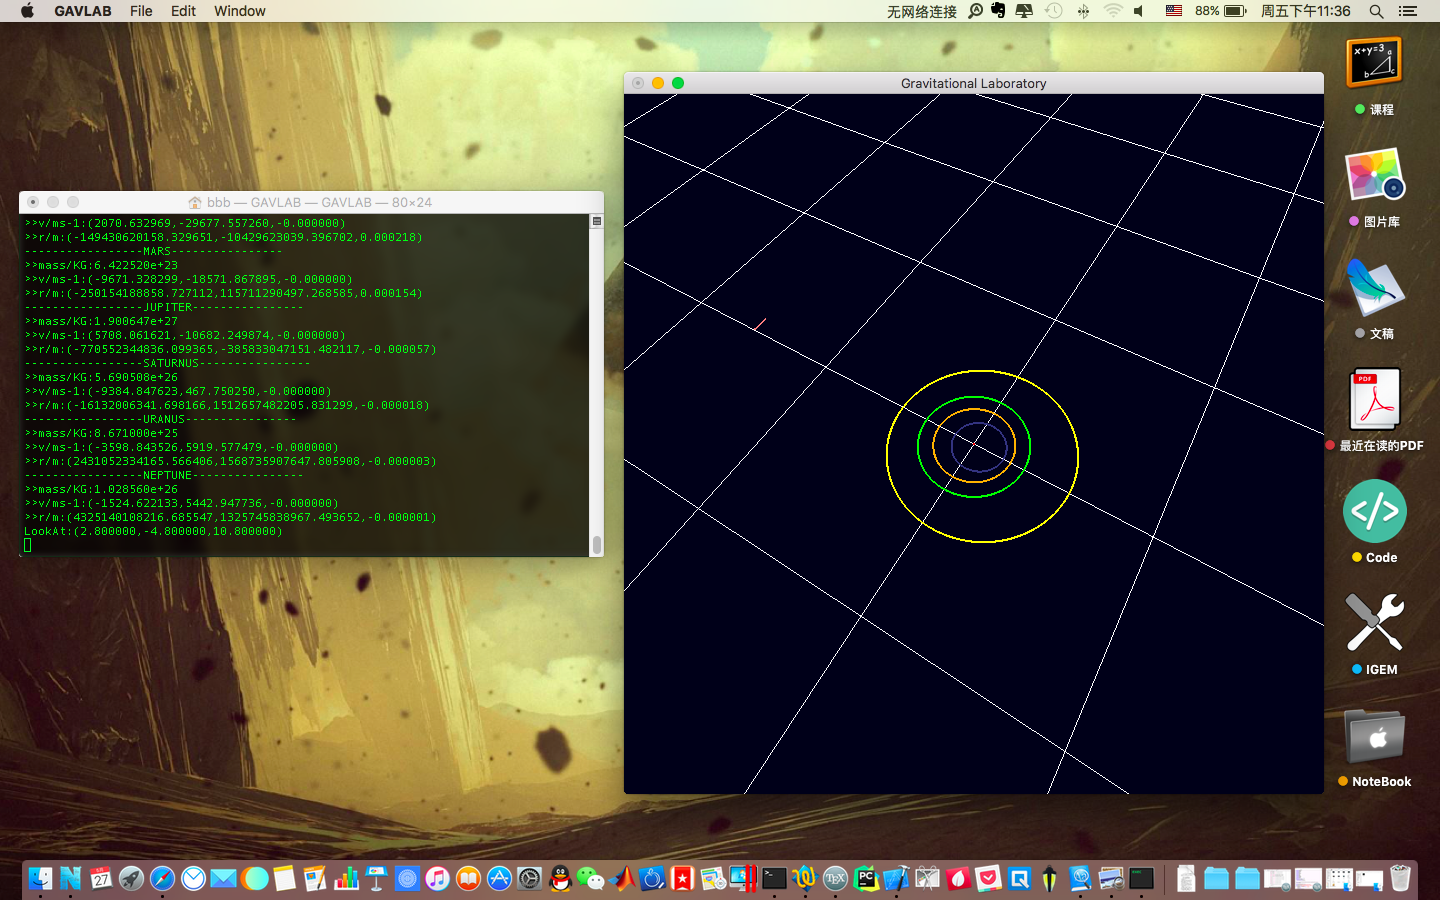
\includegraphics[width=14.4cm,height=9cm]{SI4.png}
\caption{GAVLAB is simulating solar system with SI4}
\end{figure}

So it's clearly that SI4 can handle the gravitational system simulation.
The trajectory of mercury venus and earth can maintain perfect ellipse after long time.

\clearpage
\subsubsection{CSI6}
This is the definition of class CSI6
\begin{lstlisting}[caption=CSI6 class]
class CSI4:public CIntegrator{
public:
    void Update(CSolar &S);
};
\end{lstlisting}

The formula of SI6 was derived by Yoshida\cite{SI6} in 1990 and the difference equation is
\begin{equation}
\begin{aligned}
q^i &= q^{i-1} + \tau c_{i} \frac{\partial T}{\partial p}\left(p^{i-1} \right) \\
p^i &= p^{i-1} - \tau d_{i} \frac{\partial V}{\partial q}\left(q^{i} \right) \quad i=1,2\dots 10
\end{aligned}
\end{equation}
here the coefficient is
\[
\begin{aligned}
x_{0}&=-\frac{\sqrt[3]{2}}{2-\sqrt[3]{2}},\quad x_{1}=\frac{1}{2-\sqrt[3]{2}}\\
y_{0}&=-\frac{\sqrt[5]{2}}{2-\sqrt[5]{2}},\quad y_{1}=\frac{1}{2-\sqrt[5]{2}}\\
d_{1}&=d_{3}=d_{7}=d_{9}=x_{1}y_{1},\quad d_{2}=d_{9}=x_{0}y_{1}\\
d_{4}&=d_{6}=x_{1}y_{0},\quad d_{5}=x_{0}y_{0}\\
c_{1}&=\frac{1}{2}d_{1},\quad c_{10}=\frac{1}{2}d_{9}\\
c_{i}&=\frac{1}{2}\left(d_{i-1}+d_{i} \right)\quad i=2,3,\dots,9
\end{aligned}
\]

\begin{lstlisting}[caption=CSI6 Part I]
void CSI6::Update(CSolar &S){
    double c[11];
    double d[11];
    d[1]=d[3]=d[7]=d[9]=-0.293667939522341;
    d[2]=d[8]=-1.99977809735512;
    d[4]=d[6]=0.337335879044682;
    d[5]=2.29714181079093;
    d[0]=d[10]=0;
\end{lstlisting}
\begin{lstlisting}[caption=CSI6 Part II]
    c[0]=0;
    c[1]=0.5*d[1];
    c[10]=0.5*d[9];
    for (int i=2; i<10; i++) {
        c[i]=(d[i-1]+d[i])/2.0;
    }
    vector<CPlanet>::iterator itri,itrj;
    for (itri = S.Stars.begin(); itri != S.Stars.end(); itri++) {
        vector3d r_[11],v_[11];
        r_[0]=itri->r;
        v_[0]=itri->v;
        for (int i=1; i<=10; i++) {
            r_[i]=r_[i-1] + DT*c[i]*v_[i-1];
            // Center gravity
            double r=r_[i].Magnitude();
            v_[i] = v_[i-1]-G*DT*d[i]*S.GetMass()*r_[i]/(r*r*r);
            if(i == 10) continue;
            // gravity between stars
            for (itrj = S.Stars.begin();itrj!= S.Stars.end(); itrj++) {
                if (itri == itrj) continue;
                vector3d rij = r_[i]-itrj->r;
                double R = rij.Magnitude();
                v_[i]-= DT*d[i]*G*itrj->GetMass()*rij/(R*R*R);
            }
        }
        itri->r = r_[10];
        itri->v = v_[10];
        itri->Updatetr(DT);
    }
    S.t+=DT; 
}
\end{lstlisting}

\subsection{How to simulate thousands of planets or more}
The integrating method introduced above do a really good job when simulating hundreds of planets.
However when the number of planets grows to thousands or more,the animation will be extremely slow.

The reason is quite simple.
When we integrating we have to update the velocity of the planets,thus we have to calculate the gravitational
force on it.
Since each two planets has the gravitational interaction,we have to calculate the gravitational force between each two planets.
So as the result if there are $N$ planets in the system,the running time for each updating step will be $O\left( N^2\right)$.
That running time will grow fast when $N$ become large.

Some better techniques must occur to solve this problem.
And the \textbf{Particle mesh technique and FFT} is one of the most used method to simulate the cluster system.
Here FFT means Fast Fourier Transformation.
So GAVLAB will use that method to simulate solar when it contains too many planets.
\subsubsection{Particle mesh technique}
To reduce the running time we must abandon some forces between some planets.
One way to do this is to divide the system into several meshes or girds with some cells
and we treat the particles in the same cell equally.

\begin{figure}[H]
\centering
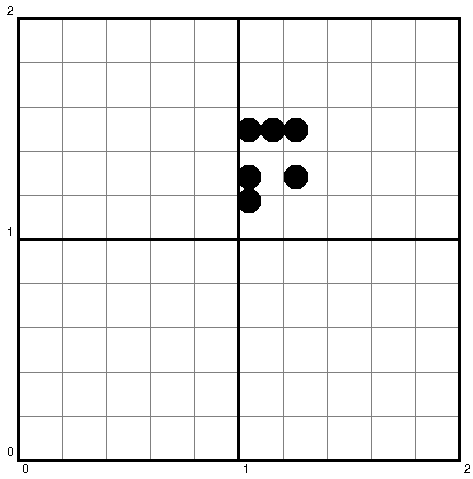
\includegraphics[width=7cm,height=7cm]{grid.pdf}
\caption{Divide the system into some cells}
\end{figure}

Then what we consider in the cell is the gravitational potential $\Phi_{\alpha}$,assuming there are $J$ cells in the grid
and the potential of cell $\alpha$ is

\begin{equation}
\Phi_{\alpha}=\sum_{\beta=1}^{J}g_{\alpha , \beta}M_{\beta}
\end{equation}
here $M_{\beta}$ is the total mass of the cell $\beta$ and $g_{\alpha , \beta}$ is the gravitational potentail between 
cell $\beta$ and $\alpha$ for unit mass.So we can get

\begin{equation}
g_{\alpha , \beta}=-\frac{G}{\sqrt{\left( \vec{r_{\alpha}} -\vec{r_{\beta}} \right)^2}}
\end{equation}

After we get our potentail of each cell in the grid we can get the difference equation on each planet in each cell

\begin{equation}
\begin{aligned}
V_{x}\left( t+\frac{1}{2}\tau  \right) &= V_{x}\left( t-\frac{1}{2}\tau  \right) + \frac{1}{2}\left(\Phi_{p+1,q,r}-\Phi_{p-1,q,r} \right) \\
V_{y}\left( t+\frac{1}{2}\tau  \right) &= V_{y}\left( t-\frac{1}{2}\tau  \right) + \frac{1}{2}\left(\Phi_{p,q+1,r}-\Phi_{p,q-1,r} \right) \\
V_{z}\left( t+\frac{1}{2}\tau  \right) &= V_{z}\left( t-\frac{1}{2}\tau  \right) + \frac{1}{2}\left(\Phi_{p,q,r+1}-\Phi_{p,q,r-1} \right) 
\end{aligned}
\end{equation}
and
\begin{equation}
\begin{aligned}
x\left(t+\tau \right) &= x\left(t \right) + V_{x}\left(t+ \frac{1}{2}\tau \right)\tau \\
y\left(t+\tau \right) &= y\left(t \right) + V_{y}\left(t+ \frac{1}{2}\tau \right)\tau \\
z\left(t+\tau \right) &= z\left(t \right) + V_{z}\left(t+ \frac{1}{2}\tau \right)\tau 
\end{aligned}
\end{equation}

It's worth to realize that GAVLAB used the simplest Euler's method to integrate which is extremely un stable.
However when there are so many planets in the system probably there will not be stable trajectory here and accuracy is
not as worth as time.

\subsubsection{Using FFT to calculate potential}
We can directly calculate $g$ but we have to calculate a lot of square roots which is slow.
So GAVLAB used FFT to calculate that.

The mechanism of FFT is a liite similar to the the mechanism of calculating the sum of logarithm to get the product
of bases.

If the solar system was divided by the $(n+1)\times (n+1) \times (n+1)$ grid,then we need $(2n \times 2n \times 2n) $ grid to do FFT.
For convenience we write $\Phi$ in position$(\alpha , \beta , \gamma)$ as
\begin{equation}
\Phi\left(\alpha , \beta , \gamma \right) = \sum_{p=0}^{2n-1} \sum_{q=0}^{2n-1} \sum_{r=0}^{2n-1} M(p,q,r) g\left(\alpha - p,\beta - q,\gamma - r \right)
\end{equation}
here
\begin{equation}
\begin{aligned}
g\left(i,j,k \right) &=-\frac{G}{\sqrt{(i \Delta_{x})^2 + (j \Delta_{y})^2 + (k \Delta_{z})^2}} \\
g\left(0,0,0 \right) &=1
\end{aligned}
\end{equation}
$g$ is Green function and $\Delta$ is the interval of the grid.

So the Fourier Transformation of the function $g$ is
\begin{equation}
\hat{g}(k,l,m) = \sum_{a=0}^{2n-1} \sum_{b=0}^{2n-1} \sum_{c=0}^{2n-1} g(a,b,c)e^{-\frac{2 \pi i}{2n}(ak+bl+cm)}
\end{equation}

\begin{equation}
\Phi \left(\alpha , \beta , \gamma \right) = \sum_{p=0}^{2n-1} \sum_{q=0}^{2n-1} \sum_{r=0}^{2n-1} M(p,q,r) (\frac{1}{2n})^3   
\sum_{k=0}^{2n-1} \sum_{l=0}^{2n-1} \sum_{m=0}^{2n-1} \hat{g}(k,l,m)e^{-\frac{2 \pi i}{2n}\left[(\alpha-p)k+(\beta - q)l+(\gamma - r)m\right]}
\end{equation}

If we change the position of the terms in the equation above we can get

\begin{equation}
\Phi \left(\alpha , \beta , \gamma \right) = (\frac{1}{2n})^3  \sum_{k=0}^{2n-1} \sum_{l=0}^{2n-1} \sum_{m=0}^{2n-1} \hat{g}(k,l,m)
\left[\sum_{p=0}^{2n-1} \sum_{q=0}^{2n-1} \sum_{r=0}^{2n-1} M(p,q,r)e^{-\frac{2 \pi i}{2n}(pk+ql+rm)} \right] e^{\frac{2 \pi i}{2n}(\alpha k + \beta l + \gamma m)}
\end{equation}

We may call the expression inside the square bracket the transformation of the mass distribution $M(p,q,r)$,let
\begin{equation}
\hat{M}(k,l,m)= \sum_{p=0}^{2n-1} \sum_{q=0}^{2n-1} \sum_{r=0}^{2n-1} M(p,q,r)e^{-\frac{2 \pi i}{2n}(pk+ql+rm)}
\end{equation}

Then $Phi$ can be expressed as
\begin{equation}
\Phi \left(\alpha , \beta , \gamma \right) = (\frac{1}{2n})^3  \sum_{k=0}^{2n-1} \sum_{l=0}^{2n-1} \sum_{m=0}^{2n-1} \hat{g}(k,l,m)
\hat{M}(k,l,m) e^{\frac{2 \pi i}{2n}(\alpha k + \beta l + \gamma m)}
\end{equation}

The whole FFT here can be written in a more concise form
\begin{equation}
\begin{aligned}
\hat{\Phi}(k,l,m) &= \hat{g}(k,l,m) \hat{M}(k,l,m) \\
\Phi(\alpha , \beta , \gamma) &= (\frac{1}{2n})^3 \sum_{k=0}^{2n-1} \sum_{l=0}^{2n-1} \sum_{m=0}^{2n-1} \hat{\Phi}(k,l,m)e^{\frac{2 \pi i}{2n}(\alpha k + \beta l + \gamma m)}
\end{aligned}
\end{equation}

This is the algorithm of FFT above
\begin{algorithm}[h]
\caption{FFT}
\KwIn{The grid}
\KwOut{$\Phi (i,j,k)$}
calculate Green function $g(a,b,c)$ of the grid\;
Fourier Transformation $g(a,c,b) \Longrightarrow \hat{g}(k,l,m)$ \;
Fourier Transformation $M(p,q,r) \Longrightarrow \hat{M}(k,l,m)$ and store that information
in $(2n \times 2n \times 2n)$ grid.\;
calculate the multiplication $\hat{\Phi}(k,l,m) \leftarrow \hat{g}(k,l,m) \hat{M}(k,l,m)$\;
final Fourier Transformation $\Phi(\alpha , \beta , \gamma) \leftarrow (\frac{1}{2n})^3 \sum_{k=0}^{2n-1} \sum_{l=0}^{2n-1} \sum_{m=0}^{2n-1} \hat{\Phi}(k,l,m)e^{\frac{2 \pi i}{2n}(\alpha k + \beta l + \gamma m)}$\;
return $\Phi$\;
\end{algorithm}

\subsubsection{CGrid class}
This is the definition of CGrid class
\begin{lstlisting}[caption=CGrid class]
class CGrid:public CIntegrator{
public:
    CGrid();
    virtual void Update(CSolar &S);
private:
    list<CPlanet> Cell[N][N][N];
    double Phi[N+2][N+2][N+2];
    void FFT();
    void UpdateCells();
    
};
\end{lstlisting}
here we have list array \textbf{Cells} to represent the cells in the grids.
\textbf{Phi} array is to store the potential array.
In each loop of simulation,firstly we call the function \textbf{UpdateCells} to
update the planets in each cell because planets will move around.
Then we call function \textbf{FFT} to update the potential array using FFT technique.
 
First we have to initialize all the array and lists of CGrid so we defined the constructor
\begin{lstlisting}[caption=CGrid()]
CGrid::CGrid(){
    for (int i=0; i<N; i++) {
        for (int j=0; j<N; j++) {
            for (int k=0; k<N; k++) {
                Cell[i][j][k].clear();
                Phi[i][j][k]=0;
            }
        }
    }
}
\end{lstlisting}

Then we update the cells by list operations
\begin{lstlisting}[caption=UpdateCells() I]
void CGrid::UpdateCells(){
    for (int i=0; i<N; i++) {
        for (int j=0; j<N; j++) {
            for (int k=0; k<N; k++) {
                list<CPlanet>::iterator itr;
                for (itr = Cell[i][j][k].begin(); itr != Cell[i][j][k].end(); itr++) {
                    // calculate the index in the grid
                    int x=itr->X()/DELDA,y=itr->Y()/DELDA,z=itr->Z()/DELDA;
                    if (x != i || y != j || z != k) {
\end{lstlisting}
\begin{lstlisting}[caption=UpdateCells() II]
                        // if the planet is out of the cell,erase it
                        Cell[i][j][k].erase(itr);
                        // and put it into right place
                        Cell[x][y][z].push_back(*itr);
                    }
                }
            }
        }
    }
}

\end{lstlisting}

This is the Update() function 
\begin{lstlisting}[caption=Update() I]
void CGrid::Update(CSolar &S){
    // Update the cells according to the position of planets
    UpdateCells();
    // using FFT to calculate potential distribution
    FFT();
    
    for (int i=0; i<64; i++) {
        for (int j=0; j<64; j++) {
            for (int k=0; k<64; k++) {
                list<CPlanet>::iterator itr;
                for (itr = Cell[i][j][k].begin(); itr != Cell[i][j][k].end(); itr++){
                   
\end{lstlisting}
\clearpage
\begin{lstlisting}[caption=Update() II]
                    double vx=(Phi[i+1][j][k]-Phi[i][j][k])
                    ,vy=(Phi[i][j+1][k]-Phi[i][j][k]),
                    vz=(Phi[i][j][k+1]-Phi[i][j][k]);
                    itr->v+=vector3d(vx,vy,vz);
                    itr->r+=DT*itr->v;
                    itr->Updatetr(DT);
                
                }
            }
        }
    }
    S.t+=DT;   
}
\end{lstlisting}

Unfortunately Particle mesh method doesn't work well either,because it used too much cells in 3-dimensional space.
Here in GABLAB I divided the grid into $64^3$ cells.
It's huge,but still not huge enough.
Usually grid method was used to research the 2-dimensional cluster system.
Grids with $256^2$ cells do a good job.
\clearpage
%>>>>>>>>>>>>>
\subsection{What if collision happens}
Well I have to say there will be a lot of collisions in the gravitational system
since the planets tend to attract each other.
So we have to decide what to do when collision happens.

In GAVLAB collisions are divided into two different circumstances.

The first case is when planet collides with sun.
Wow this is extremely dangerous and horrible so we let that planet destroyed and we add that
planet's mass onto sun's mass.
\begin{lstlisting}[caption=collision with sun]
    vector<CPlanet>::iterator itri,itrj;
    for (itri=Stars.begin(); itri != Stars.end(); itri++) {
        if (itri->exist == false) {
            continue;
        }
        double R0=(itri->r^(itri->v/(itri->v.Magnitude()))).Magnitude();
        
        if (R0<E) { // E is marco defined
            cout<<itri->Name<<" BOOM"<<endl;
            itri->exist=false;
            centerStarMass+=itri->GetMass();
        }
    }
\end{lstlisting}
\clearpage
The second case is when two close planets collides together.
When that happens we choose to merge them which means they sticked to a new planet.
According to the conservation of momentum we have
\begin{equation}
\begin{aligned}
M^\prime &= M_{1}+M_{2}\\
\vec{v^\prime} &= \frac{ M_{1}\vec{v_{1}} + M_{2}\vec{v_{2}}  }{M_{1}+M_{2}}
\end{aligned}
\end{equation}
and then we mark one of those two planet as not exist.
\begin{lstlisting}[caption=collision between planets]
vector<CPlanet>::iterator itri,itrj;
for (itri=Stars.begin(); itri != Stars.end(); itri++) {
	for (itrj=Stars.begin(); itrj!=Stars.end(); itrj++) {
        if (itrj == itri || itrj->exist==false) {continue;}
        vector3d rij=itri->r-itrj->r;
        double R=rij.Magnitude();
        if(R < E){// if they are too close
            cout<<itri->Name<<" and "<<itrj->Name<<" BOOM!"<<endl;
            // update v
            itri->v=(itri->Mass*itri->v+itrj->Mass*itrj->v)/(itri->Mass+itrj->Mass);
            itri->Mass+=itrj->Mass;// merge mass
            itrj->exist=false;// delete one of them
        }
    }
}
\end{lstlisting}



\begin{figure}[H]
\centering
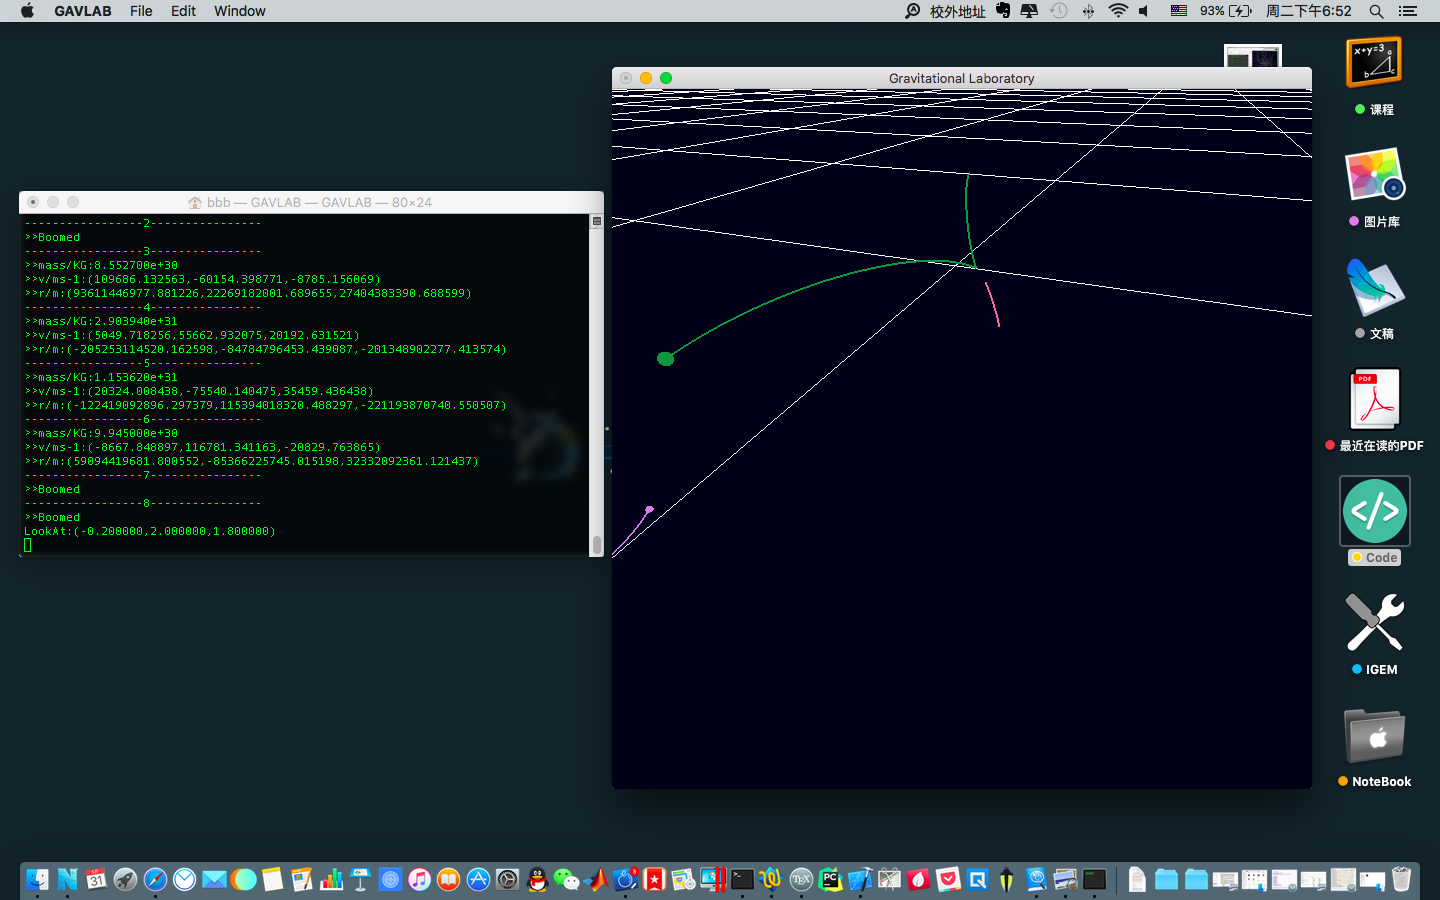
\includegraphics[width=14.4cm,height=9cm]{collision.png}
\caption{Collision happened between the green planet and the pink planet}
\end{figure}

\clearpage

\section{VIEW the GAVLAB with OpenGL}
%>>>>>>>>>>>>>
\subsection{OpenGL Library}
OpenGL is Open Graphics Library,a powerful cross platform graphic library.
It's easy to make high quality animation or graph in a short time with OpenGL.
%>>>>>>>>>>>>>
\subsection{CDisplay class}
CDisplay class integrated almost all OpenGL related code and contains two functions \textbf{display} and \textbf{reshape}
which is used to pass to the OpenGL commands 
\begin{lstlisting}[caption=CDisplay]
class CDisplay{
public:
    // draw everything
    static void display(void);
    // reshape the window when it changes size
    static void reshape (int w, int h);
private:
    // parameters for LookAt
    static GLdouble eyeX, eyeY, eyeZ;
    static GLdouble centerX, centerY, centerZ;
    static GLdouble upX, upY, upZ;
    // scale factor of LookAt parameters
    static double g;
    // position to draw the point
    static GLdouble poX;
    static GLdouble poY;
    static GLdouble poZ;
    friend class CControl;
};
\end{lstlisting}

eyeX,eyeY,eyeZ are the position of the camera
 and centerX,centerY,centerZ are the position that the camera is looking at
 and upX,upY,upZ is the direction of the up of the camera to determine the orientation of camera.
 g is the scale factor to adjust the offset.
 poX,poY,poZ is the point to be drawn

Function reshape() is called when users want to change the windos size.
\begin{lstlisting}[caption=reshape()]
void CDisplay::reshape (int w, int h){
    glViewport (0, 0, (GLsizei) w, (GLsizei) h);
    glMatrixMode (GL_PROJECTION);
    glLoadIdentity ();
    glFrustum (-1.0, 1.0, -1.0, 1.0, 1.5, 200.0);
    glMatrixMode (GL_MODELVIEW);
    glLoadIdentity();
    glTranslatef(0.0f,-20.0f,-150.0f);
}
\end{lstlisting}

Function display() is very long because it is responsible for graphing the whole system
including balls represent planet,lines represent trajectory and grids represent the coordinate.
PartI shows how to initialize gl before drawing.
\begin{lstlisting}[caption=display() PartI Set up the graph ]
void CDisplay::display(void){
    glClear(GL_COLOR_BUFFER_BIT  |  GL_DEPTH_BUFFER_BIT);
    // set the background color deep blue
    glClearColor(0, 0, 0.1, 1);
    glShadeModel (GL_SMOOTH);
    glPushMatrix();
    glMatrixMode(GL_PROJECTION);
    glLoadIdentity();
    gluPerspective(75.0f, 1.0f, 1.0f, 40000000);
    glMatrixMode(GL_MODELVIEW);
    glLoadIdentity();
    gluLookAt(eyeX, eyeY,eyeZ, centerX, centerY, centerZ, upX, upY, upZ);
    // ... the rest parts
    glPopMatrix();
    glFlush ();
}
\end{lstlisting}
\clearpage

Then we have to draw the backgrounds.
First we want to draw the 2-dimensional grids represent the reference coordinate.
Then we have to draw the sun which is fixed on origin position (0,0,0).
\begin{lstlisting}[caption=display() PartII drawing background]
void CDisplay::display(void){
    // Part I...
    //coordinate lines
    glColor3f( 1.0f, 1.0f, 1.0f );
    glLineWidth(0.1);
    // x-axis
    for(int y=-300;y<=300;y+=5){
        glBegin( GL_LINE_STRIP );
        {
            glVertex3f( -300.0f, y, 0.0f);
            glVertex3f( 300.0f, y, 0.0f);
        }
        glEnd();
    }
    // y-axis
    for(int x=-300;x<=300;x+=5){
        glBegin( GL_LINE_STRIP );
        {
            glVertex3f( x, -300.0f, 0.0f);
            glVertex3f( x, 300.0f, 0.0f);
        }
        glEnd();
    }
    // the red sun
    glColor3f(1.0, 0.0, 0.0);
    glutSolidSphere(.03, 100, 100);
    //...
}
\end{lstlisting}

\begin{figure}[H]
\centering
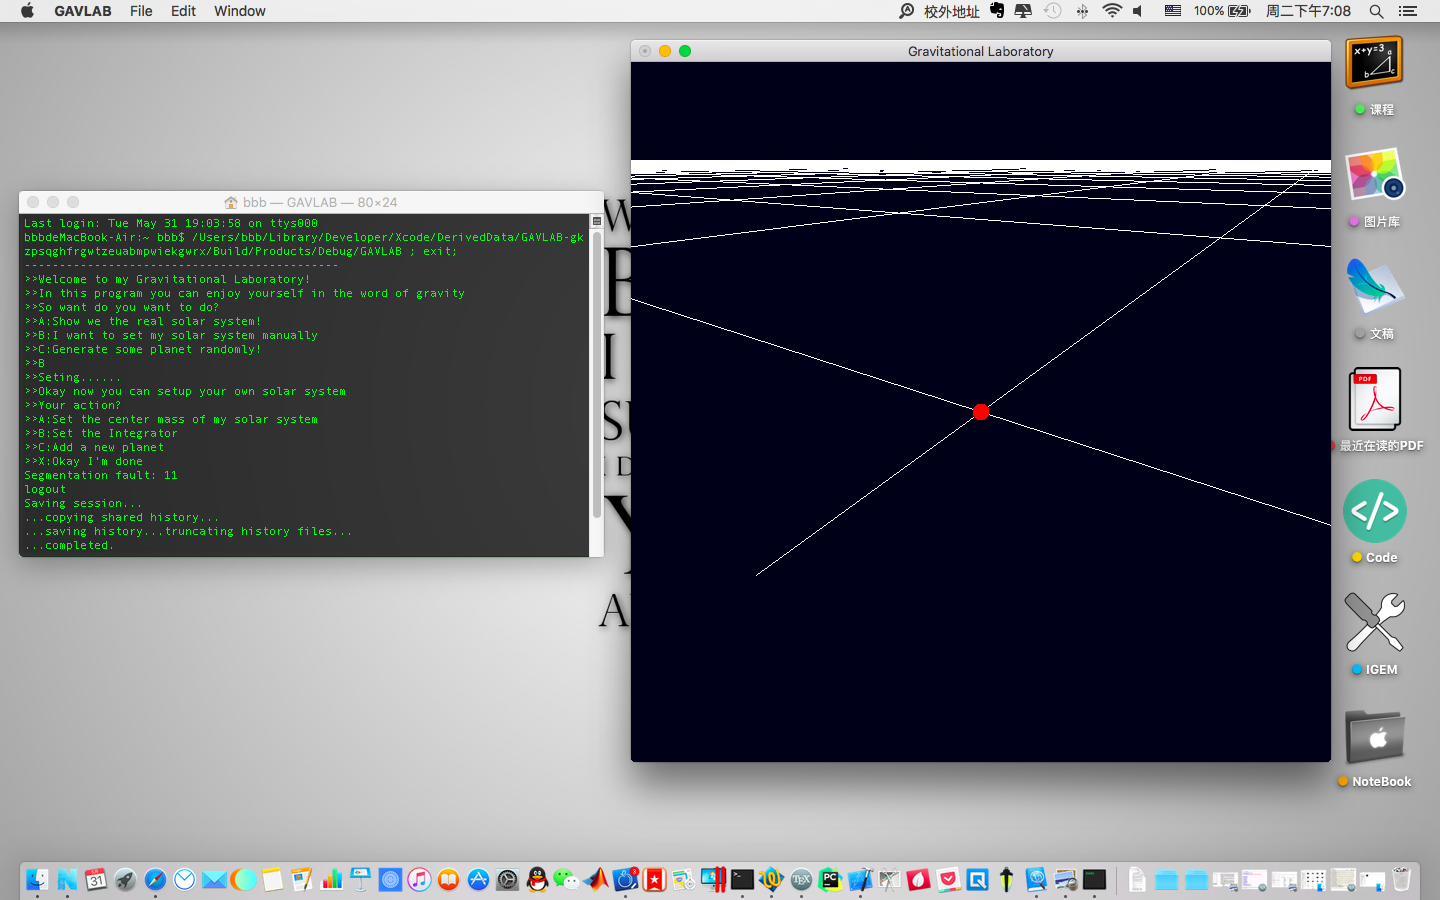
\includegraphics[width=14.4cm,height=9cm]{background.png}
\caption{Draw the background first}
\end{figure}

\clearpage
 
After that we want to draw the trajectory of all the planets cause that's what we really care about.
\begin{lstlisting}[caption=display() Part III drawing the trajectory]
void CDisplay::display(void){
    // Part I & Part II...
    vector<CPlanet>::iterator itr;
    // draw the tragetory here
    for (itr=Solar.Stars.begin(); itr != Solar.Stars.end(); itr++) {
        GLfloat r=itr->Red(),g=itr->Green(),b=itr->Blue();
        glColor3f( r, g, b );//setup the color of line
        glLineWidth(2);// make the trajectory thick 
        // this mode allows users draw stripes 
        glBegin(GL_LINE_STRIP);
        {
            list<vector3d>::iterator p;
            for (p=itr->trail.begin(); p != itr->trail.end(); p++) {
                poX = p->X()/SCALE;
                poY = p->Y()/SCALE;
                poZ = p->Z()/SCALE;
                glVertex3d(-poX,poY,poZ);
            }
        }
        glEnd();
    }
    //...
}
\end{lstlisting}
\clearpage

Some times we need not only the animation but also the real data.
For this reason GAVLAB has the option of exporting data on the command window.
\begin{lstlisting}[caption=display() PartIV exporting data]
void display(void){//Part I II III...
    if (CControl::ShowRecord == true && CControl::play == true) {
        printf("\n\n\n>>Time/DAY:%lf\n",Solar.GetT()/DAY);
    }
    for (itr=Solar.Stars.begin(); itr != Solar.Stars.end(); itr++) {
        if (itr->Exist() == false) {
            if (CControl::ShowRecord == true && CControl::play == true) {
                printf("-----------------%s----------------\n",itr->GetName().c_str());printf(">>Boomed\n");
            }continue;  
        }
        if(CControl::ShowRecord == true && CControl::play == true){
            printf("-----------------%s----------------\n",itr->GetName().c_str());
            printf(">>mass/KG:");
            printf("%e\n",itr->GetMass()*1e18);
            printf(">>v/ms-1:");
            printf("(%lf,%lf,%lf)\n",itr->GetV().X(),itr->GetV().Y(),itr->GetV().Z());
            printf(">>r/m:");
            printf("(%lf,%lf,%lf)\n",itr->X(),itr->Y(),itr->Z());
        }
    }
//...}
\end{lstlisting} 
The reason why we used C styled function printf() here instead of cout is that printf is fast while
ostream object operation cause a lot of time.
Time is everything in GAVLAB!

Finally We can draw a ball representing the planet to make GAVLAB beautiful.
\begin{lstlisting}[caption=display() Part V drawing planets]
void display(){
    // Part I-IV ...
    vector<CPlanet>::iterator itr;
    for (itr=Solar.Stars.begin(); itr != Solar.Stars.end(); itr++){
        GLfloat r=itr->Red(),g=itr->Green(),b=itr->Blue();
        double radius=0.03*itr->GetRadius();
        glColor3f(r, g, b);
        poX = itr->X()/SCALE;
        poY = itr->Y()/SCALE;
        poZ = itr->Z()/SCALE;
        // translate the position of sphere
        glTranslated(-poX,poY,poZ);
        glutSolidSphere(radius, 100, 100);
        // translate the position back to origin
        glTranslated(poX,-poY,-poZ);
    }
}
\end{lstlisting}

Because \textbf{glutSolidShpere()} can only draw sphere in position (0,0,0).
So we have to translate the origin position to the position of the planet then draw the sphere.
After that we have to translate it back in avoid of drawing the next planet in a wrong position.

\clearpage
\section{CONTROL class is the commander}
%>>>>>>>>>>>>>
\subsection{CControl class}
CControl class has two jobs.

The first job is to interact with users through command window.
It means CControl has to be able to get the command entered by users through commmand window.

The second job is to control the rest classes,functions,variables in the program such as setup the solar
system or readjust the camera.

\begin{lstlisting}[caption=CControl class]
class CControl{
public:
    static void UpdateState();
    // readjust lookAt parameter 
    static void keyboard(unsigned char key, int x, int y);
    // initialize the program
    static void init();
    // initialize the real solar
    static void initSolar();
    static void SetSolarManually();
    static void AddNewPlanet();
    static void AddRandomPlanet();
    static void Terminate();
private:
    static bool ShowRecord;// if export data
    static bool play;// is is playing or paused
    
    friend class CDisplay;

};

bool CControl::ShowRecord=false;
bool CControl::play=true;
\end{lstlisting}
\clearpage
We need a ultimate update command function.
So we defined UpadteState() function in CControl
to be the interface of all simulation related functions.
\begin{lstlisting}[caption=UpdateState()]
void CControl::UpdateState(){
    if(play)
        Solar.UpdateSolar();
    glutPostRedisplay();   
}
\end{lstlisting}

We may want to change the perspective when running GAVLAB to get a better view of 
the trajectories or want to pause simulation to find out some secret.
So want CControl does here is getting the command from the keyboard and
parse the command into operations.
\begin{lstlisting}[caption=keyboard() Part I]
void CControl::keyboard(unsigned char key, int x, int y){
    switch (key)    {
        case '+': CDisplay::g*=10; break;
        case '-': CDisplay::g/=10.0; break;
        case 'w': CDisplay::eyeY += CDisplay::g*OFFSET; break;
        case 'x': CDisplay::eyeY -= CDisplay::g*OFFSET; break;
        case 'a': CDisplay::eyeX -= CDisplay::g*OFFSET; break;
        case 'd': CDisplay::eyeX += CDisplay::g*OFFSET; break;
        case 's': CDisplay::eyeZ -= CDisplay::g*OFFSET; break;
        case 'S': CDisplay::eyeZ += CDisplay::g*OFFSET; break;
\end{lstlisting}
\clearpage
\begin{lstlisting}[caption=keyboard() Part II]
        case 'l': CDisplay::centerX -= 0.5*CDisplay::g*OFFSET; break;
        case 'j': CDisplay::centerX += 0.5*CDisplay::g*OFFSET; break;
        case 'i': CDisplay::centerY += CDisplay::g*OFFSET; break;
        case 'k': CDisplay::centerY -= CDisplay::g*OFFSET; break;
        case 'r':
            CDisplay::eyeX = 2.8; CDisplay::eyeY = 1.4; CDisplay::eyeZ= 2.4;
            CDisplay::centerX= 0; CDisplay::centerY= 0; CDisplay::centerZ= 0;
            CDisplay::upX= 0; CDisplay::upY= 0; CDisplay::upZ= 1;
            break;
        case 27: Terminate(); break;
        case ' ':play = !play;break;
        default: break;
    }
    if(ShowRecord == true){
        printf("LookAt:(%lf,%lf,%lf)\n",CDisplay::eyeX,CDisplay::eyeY,CDisplay::eyeZ);
    }
    
}
\end{lstlisting}

When users run GAVLAB the function \textbf{init()} will be called to set up all the initial variables such as 
solar system and integrators and so on.
So want init() do is getting command from the commmand window and call the interfaces of initializing functions.

Attention there used to be a lot of dialogs in printf() functions.
I just omitted those dialogs and marked them as comments.
Also I used function \textbf{usleep()} to pause between the sentences in order to
make time for users to read the word exported from command window.
\clearpage
\begin{lstlisting}[caption=init()]
void CControl::init(){
    Solar.Stars.clear();
    // dialogs and ask users want to do
    string command;
    cin>>command;
    switch (command[0]) {
        case 'A':
            CControl::initSolar();
            break;
        case 'B':
            CControl::SetSolarManually();
            break;
        case 'C':
            CControl::AddRandomPlanet();
            break;
        default:
            break;
    }
    
    printf(">>Do you want the data exported in command window?\n");
    printf(">>A:Yes\n>>B:No\n>>");
    cin>>command;
    switch (command[0]) {
        case 'A':
            CControl::ShowRecord=true;
            break;
        case 'B':
            CControl::ShowRecord=false;
            break;
        default:
            break;
    }
    // dialogs and tell users how to operate GAVLAB
}
\end{lstlisting}
\clearpage

The first choice for users is to simulate the real solar system!
So we have to initial the solar system before simulation,add real planets's data into the Solar object.
When simulating real solar,we just use SI4 integrator.
\begin{lstlisting}[caption=initSolar()]
void CControl::initSolar(){
    printf(">>Please wait...\n");
    double dt=DAY*0.1;
    Solar.SetMass(MS);
    Solar.SetI(SI4);
    Solar.SetStep(dt);
    CPlanet mercuy("MERCURY",0.0553*ME,0.35,0.3871*RA,0,344,0,52716.3,0,.2, .2, .5);
    CPlanet venus("VENUS",0.815*ME,0.8,0.7233*RA,0,0,0,35200,0, 1, .7, 0);
    CPlanet earth("EARTH",ME,0.8,RA,0,0,0,29789,0, 0, 1, 0);
    CPlanet mars("MARS",0.1074*ME,3,1.523*RA,0,0,0,25310,0, 1, 1, 0);
    CPlanet jupiter("JUPITER",317.834*ME,2.5,5.202*RA,0,0,0,13413,0, 1, .5, .5);
    CPlanet saturnus("SATURNUS",95.159*ME,1.5,9.544*RA,0,0,0,9927.7,0, 1, 1, .5);
    CPlanet uranus("URANUS",14.5*ME,1.5,19.19*RA,0,0,0,6978,0, .5, 1, .5);
    CPlanet neptune("NEPTUNE",17.2*ME,0.35,30.13*RA,0,0,0,5670.9,0, .4, .4, .4);
    Solar.AddPlanet(mercuy);
    Solar.AddPlanet(venus);
    Solar.AddPlanet(earth);
    Solar.AddPlanet(mars);
    Solar.AddPlanet(jupiter);
    Solar.AddPlanet(saturnus);
    Solar.AddPlanet(uranus);
    Solar.AddPlanet(neptune);
    printf(">>done\n");
}
\end{lstlisting}
\clearpage

Also GAVLAB is a program with freedom which means the users can add any planet in the solar.
Then function \textbf{SetSolarManually()} will be called and ask users to enter the data through
command window.

\begin{lstlisting}[caption=SetSolarManually()]
void CControl::SetSolarManually(){
    
    printf(">>Seting......\n");
    usleep(3000000);
    printf(">>Okay now you can setup your own solar system\n");
    usleep(1000000);
    printf(">>Your action?\n");
    printf(">>A:Set the center mass of my solar system\n");
    printf(">>B:Set the Integrator\n");
    printf(">>C:Add a new planet\n");
    printf(">>X:Okay I'm done\n");
    string command;
    string IntrgratorType;
    bool Ismass=false,IsIntegrator=false;
    bool isbreak=false;
    while (cin>>command) {
        switch (command[0]) {
       // switch the command showed in CODE 37-38
        }
        if (isbreak) {
            break;
        }
        printf(">>Your action?\n");
        printf(">>A:Add a new planet\n");
        printf(">>B:Okay I'm done\n");
        
    }
}
\end{lstlisting}
\clearpage

\begin{lstlisting}[caption=switch part I]
        switch (command[0]) {
            case 'A':
                double Mass;
                printf(">>Mass/kg:");
                cin>>Mass;
                Solar.SetMass(Mass);
                Ismass = true;
                break;
            case 'B':
                printf(">>You can choose the following Integrators\n");
                printf(">>A:SI2\n>>B:SI4\n>>C:SI6\n>>D:Grid\n>>");
                cin>>IntrgratorType;
                switch (IntrgratorType[0]) {
                    case 'A':
                        Solar.SetI(SI2);
                        IsIntegrator=true;
                        break;
                    case 'B':
                        Solar.SetI(SI4);
                        IsIntegrator=true;
                        break;
                    case 'C':
                        Solar.SetI(SI6);
                        IsIntegrator=true;
                        break;
                    case 'D':
                        Solar.SetI(Grid);
                        IsIntegrator=true;
                        break;
                    default:
                        break;
                }
                break;
\end{lstlisting}
\clearpage
\begin{lstlisting}[caption=switch part II]
            case 'C':
                CControl::AddNewPlanet();
                break;
            case 'X':
                if (IsIntegrator && Ismass) {
                    isbreak=true;
                }
                else{
                    if (!IsIntegrator) {
                        printf(">>You didn't set your solar's integrator\n");
                    }
                    if (!Ismass) {
                        printf(">>You didn't set your solar's center mass\n");
                    }
                }
                break;
            default:
                break;
        }
\end{lstlisting}
\clearpage

If we chose to add a planet in the solar system manually 
in function \textbf{SetSolarManually()} it will call function
\textbf{AddNewPlanet()} which will get the information from the commmand window
entered by user and then it will generate the corresponding planet and add it into solar system.\\

\begin{lstlisting}[caption=AddNewPlanet()]
void CControl::AddNewPlanet(){
    string name;
    double mass;
    double radius;
    double x,y,z,vx,vy,vz;
    double r,g,b;
    printf(">>name:");cin>>name;
    printf(">>mass/kg:");cin>>mass;mass/=1e18;
    printf(">>radius/km:");
    cin>>radius;radius/=1.4e6;
    printf(">>Assuming the sun is in (0,0,0)\n");
    printf(">>Position X/AU:");cin>>x;x*=RA;
    printf(">>Position Y/AU:");cin>>y;y*=RA;
    printf(">>Position Z/AU:");cin>>z;z*=RA;
    printf(">>Velocity Vx/ms-1:");cin>>vx;
    printf(">>Velocity Vy/ms-1:");cin>>vy;
    printf(">>Velocity Vz/ms-1:");cin>>vz;
    printf(">>Set the Color now\n");
    printf(">>Red:");cin>>r;
    printf(">>Green:");cin>>g;
    printf(">>Blue:");cin>>b;
    P = new CPlanet(name,mass,radius,x,y,z,vx,vy,vz,r,g,b);
    Solar.AddPlanet(*P);
}
\end{lstlisting}
\clearpage

Finally if the users choose to press ESC to terminate GAVLAB,function
\textbf{Terminate()} will be called.

In fact Terminate() controls what happen when the program exits.\\
\begin{lstlisting}[caption=Terminate()]
void CControl::Terminate(){
    printf(">>The simuation is over\n");
    printf(">>Thanks for using\n");
    exit(0);
}
\end{lstlisting}

\begin{figure}[H]
\centering
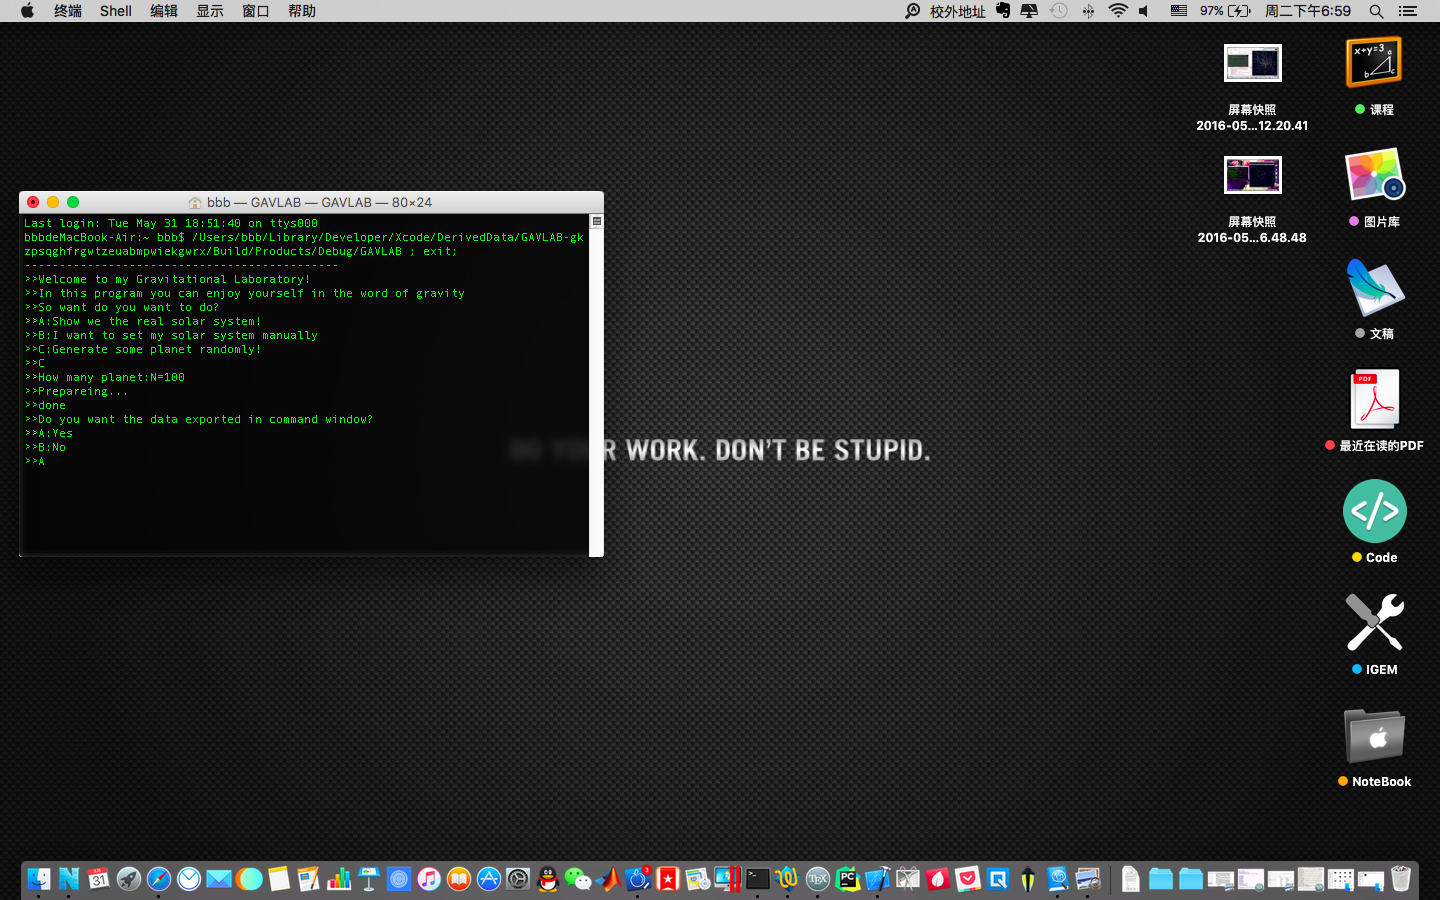
\includegraphics[width=14.4cm,height=9cm]{control.png}
\caption{CControl is asking for order}
\end{figure}
\clearpage

%>>>>>>>>>>>>>
\subsection{main function}

Finally Let's see what's happening in main function.\\
\begin{lstlisting}[caption=main()]
CSolar Solar;
CPlanet* P;
int main(int argc, char** argv) {
    CControl Control;
    Control.init();
    glutInit(&argc, argv);
    glutInitDisplayMode (GLUT_RGBA |  GLUT_SINGLE);
    glutInitWindowSize (700, 700);
    glutInitWindowPosition (700, 100);
    glutCreateWindow ("Gravitational Laboratory");
    glutDisplayFunc(CDisplay::display);
    glutReshapeFunc(CDisplay::reshape);
    glutKeyboardFunc(CControl::keyboard);
    glutIdleFunc(CControl::UpdateState);
    glutMainLoop();
    return 0;
}
\end{lstlisting}
\clearpage
I will explain those glut-prefixed functions here
\begin{description}[align=left]
\item [glutInit] initialize GLUT 
\item [glutInitDisplayMode] Set up the display mode.Here we chose RGBA color mode and single buffer window mode.
\item [glutInitWindowSize] Set the size of the window.
\item [glutInitWindowPosition] Set the position of the window.
\item [glutCreateWindow] Create a window.
\item [glutDisplayFunc] Time to display!Our CDisplay::display is the argument of this function which means when it's time to display in
a loop GAVLAB will call display function.
\item [glutReshapeFunc] Time to reshape the window and it will call our CControl::reshape function.
\item [glutKeyboardFunc] Time to parse the command from the keyboard.When users type on keyboard GAVLAB will call our CControl::keyboard function
to parse the command.
\item [glutIdleFunc] When there's no extra command GAVLAB will call function CControl::UpdateState in the loop.
\item [glutMainLoop] The whole animation is a big loop in which the functions above will be called and executed one by one.

\end{description}

And we defined a global variable Solar because there's only one solar system in GAVLAB.
The CPlanet pointer is pointing those planet objects who are dynamically allocated durring the program.
\clearpage


\section{Epilogue}
\subsection{I paid a lot of time building GAVLAB}
I've been building GAVLAB since the beginning of this semester after professor Xue assigned this project.
For days and days I cost a lot of time thinking how to build it.
At first the design and blue print was finished at April.
Then it took me half a month to program and code on my computer.
For the whole May I kept optimizing the model, restructure my program to be perfect
and test the result of GAVLAB.
At last I used three days to make this 50 pages report by \LaTeX .

All the work was done by myself,including thousands lines of code and 50 pages report.
\subsection{I found a lot of reference}
I found a lot of resources,including three books \textbf{Gravitational N-Body Simulations},
\textbf{The Computer Simulation of The Gravitational N-Body Problem } , \textbf{The Art of Molecular Dynamic Simulation}
and tens of papers from Comp Phys.

I also read \textbf{OpenGL SuperBible} to make GAVLAB visual.
\subsection{I really love GAVLAB}
\textbf{GAVLAB} is the third big C++ program I've ever built after \textbf{Pokemon} and \textbf{The Game of Brick}.
It's my own child,I really love it.
It's so beautiful,so powerful to me.
\subsection{I appreciate Professor Xue}
Thank you for giving me such a chance to experience the importance of data structure and the pleasure
of programing,especially the happiness of making my own program.



\clearpage
\begin{thebibliography}{99}
\bibitem{mathlibrary}Physics.for.Game.Developers. David.M.Bourg. 2nd 2013 111
\bibitem{SI}The computer Simulation of The Gravitational N-Body Problem LiuBulin
\bibitem{SI4}Celestial Mechanics and Dynamical Astronomy Haruo Yoshida 1993 56 27
\bibitem{SI6}Phys Letters Yoshida H A 1990,150:262
\end{thebibliography}


\end{document}


























